% vim: spelllang=fr

\documentclass[../main.tex]{subfiles}
\graphicspath{{\subfix{../Figures/Chap4/}}}
\begin{document}
\vspace{-0.5cm}

\begin{itshape}
    Dans ce dernier chapitre, nous nous intéressons à l'ajout de nouveaux prédicteurs dans des indices de cyclogénèse construits par régression de Poisson.
    L'apport de l'ajout explicite du mode de variabilité El Niño dans la régression est étudié dans un premier temps. Ensuite, nous nous intéressons au
    remplacement de l'humidité relative à \hPa{600} par une mesure intégrée sur la colonne du déficit de saturation d'humidité. Cet indice est ensuite appliqué
    à deux simulations en climat plus chaud avec le modèle ARPEGE utilisé dans sa configuration basculée-étirée.
\end{itshape}

\minitoc
\newpage

%--------------------------------------
\section{Introduction}

Le \cref{chap:chapitre_3} a porté sur la modification des coefficients $b$ du TCS pour étudier la façon dont ces coefficients affectent la variabilité
interannuelle inférée par l'indice. Plusieurs approches ont été expérimentées, telles que la réalisation de la régression sur des champs à plus haute
résolution, en introduisant de la variabilité temporelle à plus haute fréquence, ainsi qu'en réalisant des régressions locales à l'échelle des bassins
océaniques. Re-déterminer les coefficients $b$ du TCS pour obtenir un indice mieux adapté à son jeu de données, à l'échelle globale comme régionale, présente
une réelle plus-value, mais l'amélioration de la représentation de la variabilité interannuelle n'en fait cependant pas partie. Celle-ci apparaît en effet comme
particulièrement robuste aux changements dans les coefficients de l'indice, si bien que le choix des prédicteurs dans la régression apparaît comme la seule
façon d'influencer la variabilité interannuelle.

Dans ce chapitre, il s'agit par conséquent d'étudier l'apport de deux nouveaux prédicteurs dans la construction d'un indice de cyclogénèse par régression de
Poisson. Dans un premier temps, nous ajouterons explicitement un diagnostique du mode de variabilité El Niño comme nouveau prédicteur dans la régression. L'ENSO
est en effet connu pour sa modulation de l'activité cyclonique tropicale \parencite{chan_tropical_1985,landsea_ninosouthern_2000,lin_enso_2020} et constitue
une source de prévisibilité de l'activité cyclonique à l'échelle interannuelle. L'ajout d'un diagnostique ENSO dans la régression est considérée ici à titre
expérimental, car la philosophie des indices de cyclogénèse consiste habituellement à introduire les ingrédients qui sont supposés intervenir directement dans
le processus physique de cyclogénèse. L'ENSO affecte quant à lui la SST, le cisaillement vertical ainsi que l'humidité relative à différents degrés selon les
régions et par télé-connexions. Il ne s'agit donc pas d'un ingrédient intervenant directement dans le processus de formation d'un cyclone tropical. Il est
toutefois permis de penser que l'ajout de cette information de la façon la plus explicite possible dans un indice de cyclogénèse pourrait être susceptible
d'impacter de manière significative sa variabilité interannuelle.

Dans un second temps, nous remplacerons le prédicteur d'humidité, définie dans le TCS comme l'humidité relative à \hPa{600}, par le déficit de saturation
d'humidité intégré sur la colonne. Le déficit de saturation possède en effet la propriété d'évoluer avec le réchauffement climatique dans la mesure où la loi de
Clausius-Clapeyron indique que la quantité de vapeur d'eau que l'atmosphère est capable de stocker augmente à hauteur de \prct{7} par degré de réchauffement, là
où l'humidité relative est projetée comme constante. Plusieurs études suggèrent par ailleurs que le déficit de saturation est un paramètre plus pertinent que
l'humidité relative dans le processus de cyclogénèse \parencite{emanuel_hurricanes_2008,emanuel_tropical_2010}. De plus, \textcite{camargo_testing_2014}
montrent que des indices construits par régression de Poisson et utilisant cette variable en remplacement de l'humidité relative indiquent une réponse au
réchauffement climatique cohérente avec la méthode directe de détection objective dans les projections futures.

\section{Utilisation d'un indice Niño dans une régression de Poisson}\label{sec:indice_ONI}

On s'intéresse ici à l'ajout explicite du signal du mode de variabilité ENSO (\textit{El Niño-Southern Oscillation}) dans un indice de cyclogénèse construit par
régression de Poisson, dans le but de voir si cet apport d'information est susceptible d'améliorer la variabilité interannuelle inférée par l'indice.

Nous nous plaçons pour cela dans le cadre du modèle de climat ARPEGE, avec une simulation de la période historique forcée par la SST observée issue de la base
de données HadISST1. Dans la mesure où la construction de nouveaux indices de cyclogénèse a pour finalité une application à des simulations de réchauffement
climatique, il est en effet nécessaire de valider la méthodologie mise en place dans le \cref{chap:chapitre_3} avec un modèle de climat. Par ailleurs,
\textcite{camargo_testing_2014} argumentent que la construction d'indices directement sur les modèles est pertinente car la relation liant l'environnement de
grande échelle et l'activité cyclonique simulée par le modèle n'est à priori pas exactement la même que dans la réalité ---~ou du moins la réalité vue par le
prisme des réanalyses atmosphériques.

La simulation ARPEGE forcée par HadISST1 ---~décrite plus en détails dans la section suivante~--- présente donc la chronologie observée des variables de basse
fréquence issues de l'Océan, et voit notamment l'emprunte des épisodes El Niño / La Niña via les SST historiques, mais l'évolution des variables atmosphériques est
régie par le modèle ARPEGE. Cette simulation possède en outre ses propres cyclones tropicaux, différents de ceux contenus dans IBTrACS.

\subsection{Données et Méthodes}

\subsubsection{Simulation historique forcée avec ARPEGE-Climat}

Nous utilisons ici le modèle ARPEGE dans sa version 6.3 à haute résolution, dans la même configuration que dans
\textcite{chauvin_future_2020,cattiaux_projected_2020}. Cette version du modèle est quasiment identique à celle utilisée dans le modèle couplé CNRM-CM6-1
\parencite{voldoire_evaluation_2019} et CNRM-ESM2 \parencite{seferian_evaluation_2019}, participant à CMIP6 \parencite{eyring_overview_2016} et HighResMIP
\parencite{haarsma_highresmip_2020}. Une description détaillée de toutes les nouveautés dans cette version d'ARPEGE par rapport à la version précédente (5.2)
est disponible dans \textcite{voldoire_evaluation_2019}, tandis que la version précédente est décrite dans \textcite{voldoire_cnrmcm5_2013}. Nous ne précisons
alors ici que les éléments particulièrement pertinents pour la simulation des cyclones tropicaux. Ainsi, le modèle est constitué du schéma physique PCMT
(\textit{Prognostic Condensates Microphysics and Transport}), incluant le schéma convectif de \textcite{piriou_approach_2007,gueremy_continuous_2011}, offrant
une paramétrisation de la convection profonde et peu profonde. Cette version voit également l'ajout de dix nouvelles variables pronostiques\footnote{Les
variables dites \textquote{pronostiques} se distinguent des variables dites \textquote{diagnostiques} en cela que leur évolution temporelle est décrite par la
résolution d'une équation dans le modèle numérique. Par opposition, les variables diagnostiques (par exemple, l'humidité relative) sont dérivées des variables
pronostiques (température, pression, humidité spécifique...).}, en plus des six déjà présentes. Spécifiquement, ARPEGE 6.3 calcule désormais l'évolution du
contenu en eau liquide et solide, précipitée ou nuageuse, de l'énergie cinétique turbulente et de la vitesse verticale convective. La paramétrisation de la
microphysique provient du schéma de \textcite{lopez_implementation_2002}, tandis que le schéma de turbulence est issu de \textcite{cuxart_turbulence_2000}. Le
modèle possède \num{91} niveaux verticaux, jusqu'à \hPa{0.01}, et la couche de mélange atmosphérique est caractérisée par \num{15} niveaux verticaux en dessous
de \m{1500} d'altitude.

La simulation utilisée ici est une simulation historique sur la période \num{1979}~--~\num{2010} et sur une grille T359, de taille \num{720} (longitude)
$\times$ \num{360} (latitude), donc à une résolution horizontale de \ang{0.5}, soit d'environ \km{50} à l'équateur. La simulation est forcée par la SST et la concentration
en glace de mer issues d'observations et provenant de la base de données HadISST1 \parencite{rayner_global_2003}.

\subsubsection{Cylogénèses simulées}\label{sec:tracking_arpege}

Les cyclones tropicaux sont détectés à l'aide du schéma de détection du CNRM \parencite{chauvin_response_2006}, amplement décrit dans le \cref{chap:chapitre_2},
notamment dans la \cref{sec:eval_tracker_ERA5}. Le schéma de détection a été appliqué aux champs 6-horaires du modèle avec : un seuil de vorticité
\textbf{VOR}~$=$~\SI{20e-5}{\per\second} ; un seuil de vent \textbf{RES}~$=$~\ms{13}, un seuil d'anomalie de température \textbf{TANOM}~$=$~\SI{1}{\kelvin} ; un
seuil de profil vertical de température \textbf{PT}~$=$~\SI{-2}{\kelvin} ; un seuil de profil vertical de vitesse du vent \textbf{PW}~$=$~\ms{5}, et enfin un
paramètre de relaxation des trajectoires \textbf{REL} fixé à \SI{20e-5}{\per\second}. Ces paramètres se distinguent notablement de ceux utilisés pour ERA5 dans
\textcite{dulac_assessing_2023} par le seuil vorticité (respectivement \SI{15e-5}{\per\second}) et surtout par le seuil de vitesse du vent à la surface
(respectivement \ms{5}). Rappelons en effet que le modèle ARPEGE, en particulier cette version précise du modèle, est connue pour simuler des cyclones tropicaux
intenses par rapport à la résolution du modèle \parencite{roberts_impact_2020,chauvin_future_2020} (voir aussi \cref{sec:cyclones_dans_modèles} du
\cref{chap:chapitre_1}, notamment la \cref{fig:roberts_PV_resolution}, \vpageref{fig:roberts_PV_resolution}). Il convient néanmoins de préciser que
contrairement au \cref{chap:chapitre_2}, le choix des seuils de détection utilisés pour détecter les TC dans cette simulation n'ont pas fait l'objet d'une
analyse quantitative des performances ---~une telle analyse serait par ailleurs impossible étant donné qu'il n'existe pas de trajectoires de référence pour les
pures simulations atmosphériques. Avant post-traitement des trajectoires, la fréquence d'occurrence annuelle moyenne de cyclogénèses est de \num{80.7} TC par
an. À titre de référence, IBTrACS sur la même période indique \num{82.9} TC par an.

Nous appliquons en post-traitement le filtre des systèmes de moyennes latitudes basé sur le diagnostique du jet subtropical (STJ), décrit et illustré dans la
\cref{sec:filtrage_mid_latitudes} (\cref{chap:chapitre_2}). Ce filtre est choisi ici ---~en dépit des réserves exprimées dans le \cref{chap:chapitre_2}~--- en
raison de sa relative simplicité à implémenter, notamment par rapport au filtre du $V_U^T$ qui a lui été préféré dans \textcite{dulac_assessing_2023}. En effet,
l'emploi du filtre du $V_U^T$ comme post-traitement nécessite de traiter en profondeur les champs spatiaux 3D du modèle centrés sur les positions des TC
préalablement identifiés, une opération qui est à la fois techniquement complexe et chronophage. En comparaison, la détermination de la limite équatoriale du
STJ peut être faite une fois pour toutes, et n'est pas à proprement parler dépendante des trajectoires identifiées, au sens où il n'est pas nécessaire de
répéter le diagnostique pour appliquer le filtre à de nouvelles trajectoires issues de la même simulation. En outre, \textcite{bourdin_intercomparison_2022}
montrent que le filtre du STJ parvient très efficacement à filtrer les systèmes de moyennes latitudes, lorsqu'appliqué à plusieurs schémas de détection sur
ERA5. Rappelons brièvement que la latitude du STJ est déterminée en prenant la limite équatoriale des points où le module du vent à \hPa{200} (lissé sur trois
mois glissants) est supérieur à \ms{25} et où la composante zonale (lissée de la même façon) est supérieure à \ms{15}. En pratique, puisqu'on s'intéresse aux
cyclogénèses et qu'on ne garde pour cela que les premières échéances des trajectoires, le filtre consiste à retirer les points situés au delà de la latitude du
STJ.

La \cref{fig:track_density_PRE625REFT359x} présente la densité annuelle moyenne (sur \num{30} ans) des premières échéances des trajectoires détectées dans la
simulation ARPEGE ---~assimilées aux cyclogénèses~--- après application du filtre du STJ. Avec le filtre du STJ, la fréquence annuelle moyenne est réduite à
\num{60.8} TC par an. Le filtre retire en effet \num{617} cyclogénèses, mais tous ne sont pas purement extra-tropicaux car la latitude médiane des cyclogénèses
filtrées est de \ang{26.2}N dans l'hémisphère nord ($n = \num{366}$) et de \ang{31.8}S dans l'hémisphère sud ($n=251$). On note également une latitude minimale
parmi les systèmes filtrés à \ang{2}N et à \ang{8.6}S pour chacun des deux hémisphères respectifs. Le jet subtropical ne peut physiquement pas se trouver en
dessous de \ang{2}N. Ce cas illustre un des points (en l'occurence une des limitations du filtre) discuté dans la \cref{sec:filtrage_mid_latitudes} (et
parfaitement illustré sur la \cref{fig:geopdy_and_STJ}, troisième ligne, \vpageref{fig:geopdy_and_STJ}), et peut être considéré comme un effet de bord. Le
filtre parvient toutefois à supprimer \num{95} des \num{97} cyclogénèses situées au delà de \ang{40} (nord et sud) dans les trajectoires non-filtrées.

\begin{figure}[tb]
    \centering
    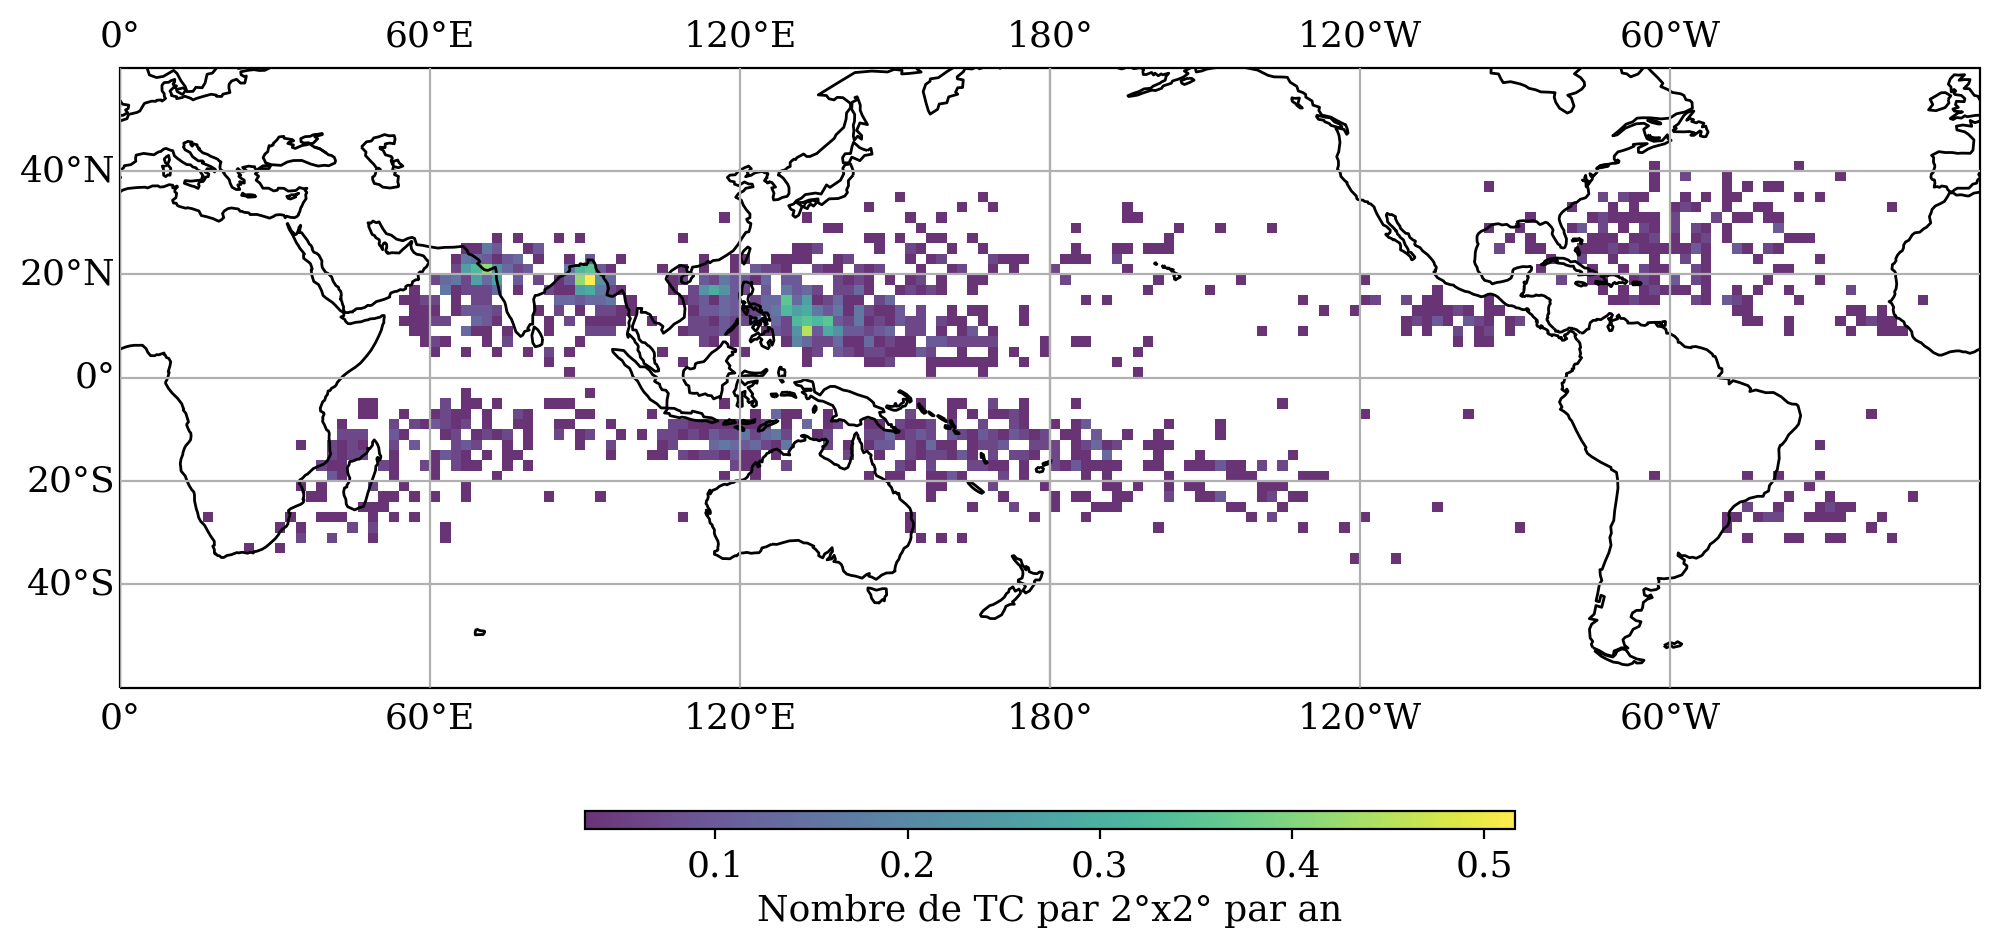
\includegraphics[width=\textwidth]{track_density_PRE625REFT359x.png}
    \caption{Densité annuelle moyenne de cyclogénèses dans la simulation ARPEGE forcée par HadISST1 entre 1980 et 2010, calculée sur une grille régulière de
    \ang{2}$\times$\ang{2}.}
    \label{fig:track_density_PRE625REFT359x}
\end{figure}

La \cref{fig:density_arpege_ibtracs} présente le biais moyen entre la simulation ARPEGE (c.f \cref{fig:track_density_PRE625REFT359x}) et IBTrACS, prise sur la
même période, en termes de densité de probabilité d'occurrence pour pallier à la différence dans la fréquence annuelle des deux jeux de données après
application du filtre du STJ. Dans l'océan Atlantique, la \cref{fig:density_arpege_ibtracs} fait apparaître une légère surestimation dans l'Atlantique Sud d'une
part, et un déséquilibre dans l'Atlantique nord avec notamment une sous-évaluation dans le MDR et le GoM, mais une sur-évaluation dans le reste de l'océan. Ce
biais dans l'atlantique nord avec cette simulation est par ailleurs documenté dans \textcite{chauvin_future_2020}. Dans le bassin EPac, l'activité simulée est
fortement sous-estimée. Dans le WPac, un surplus est noté dans ARPEGE en Mer de Chine méridionale et Mer des Philippines, tandis que le reste du bassin voit
sinon un déficit. Dans le bassin NInd, la simulation ARPEGE présente une activité sur-estimée aussi bien en Mer d'Arabie que dans le Golfe du Bengale. Dans
l'hémisphère sud, le biais est plus contrasté. Dans l'océan Indien, on note un biais positif dans le sud-ouest du bassin, autour de Madagascar mais un biais
négatif dans le nord-est, proche de l'équateur. Une répartition du biais similaire mais symétrique est notée dans le bassin Sud Pacifique, avec un biais positif
dans le sud-est et négatif au nord-ouest.

Dans la plupart des bassins, ces motifs de biais sont en fait évocateurs d'une mauvaise localisation des cyclogénèses par le schéma de détection, notamment en
raison de sa tendance connue à détecter les TC un peu tardivement, plutôt que d'un biais avéré dans l'activité simulée. Dans le NAtl, les trajectoires démarrent
le plus souvent de la MDR ou du GoM pour ensuite remonter vers le nord / nord-est. Dans le SInd, les TC se déplacent souvent du nord-est vers le sud-ouest. Le
sens de circulation est inversé dans le SPac en raison du flux de mousson en provenance d'ouest qui prend le pas sur la dérive de Coriolis ---~cette dernière
ayant naturellement tendance à déplacer les TC vers l'ouest dans l'hémisphère sud (c.f \cref{sec:conditions_cyclogenese})~--- si bien que les TC s'y déplacent
généralement vers le sud-est. Une détection trop tardive des TC pourrait également expliquer au moins en partie le biais noté dans le WPac (voir aussi
\cref{fig:bassins_TC} du \cref{chap:chapitre_1}, \vpageref{fig:bassins_TC}, pour voir les sens de déplacement des TC dans les bassins océaniques majeurs). Le
\cref{chap:chapitre_2} fait notamment référence à cette tendance que possède le schéma de détection à détecter trop tardivement les TC dans la réanalyse ERA5,
et cet effet est également documenté dans \textcite{bourdin_intercomparison_2022}. Dans ce contexte, les seules régions où il existe un biais réel entre
l'activité simulée par ARPEGE et l'activité observée (outre la différence de fréquence annuelle après passage du filtre) sont le bassin EPac, le NInd, et dans
une mesure bien moindre le Sud Atlantique. L'activité cyclonique telle que simulée dans le modèle ARPEGE et identifiée par le traqueur du CNRM est donc tout
compte fait assez fidèle aux observations. Nous considérons alors que les cyclogénèses issues du schéma de détection du CNRM appliqué à la simulation ARPEGE
peuvent être utilisées comme prédictant pour la construction d'indices de cyclogénèse par régression de Poisson.

\begin{figure}[tb]
    \centering
    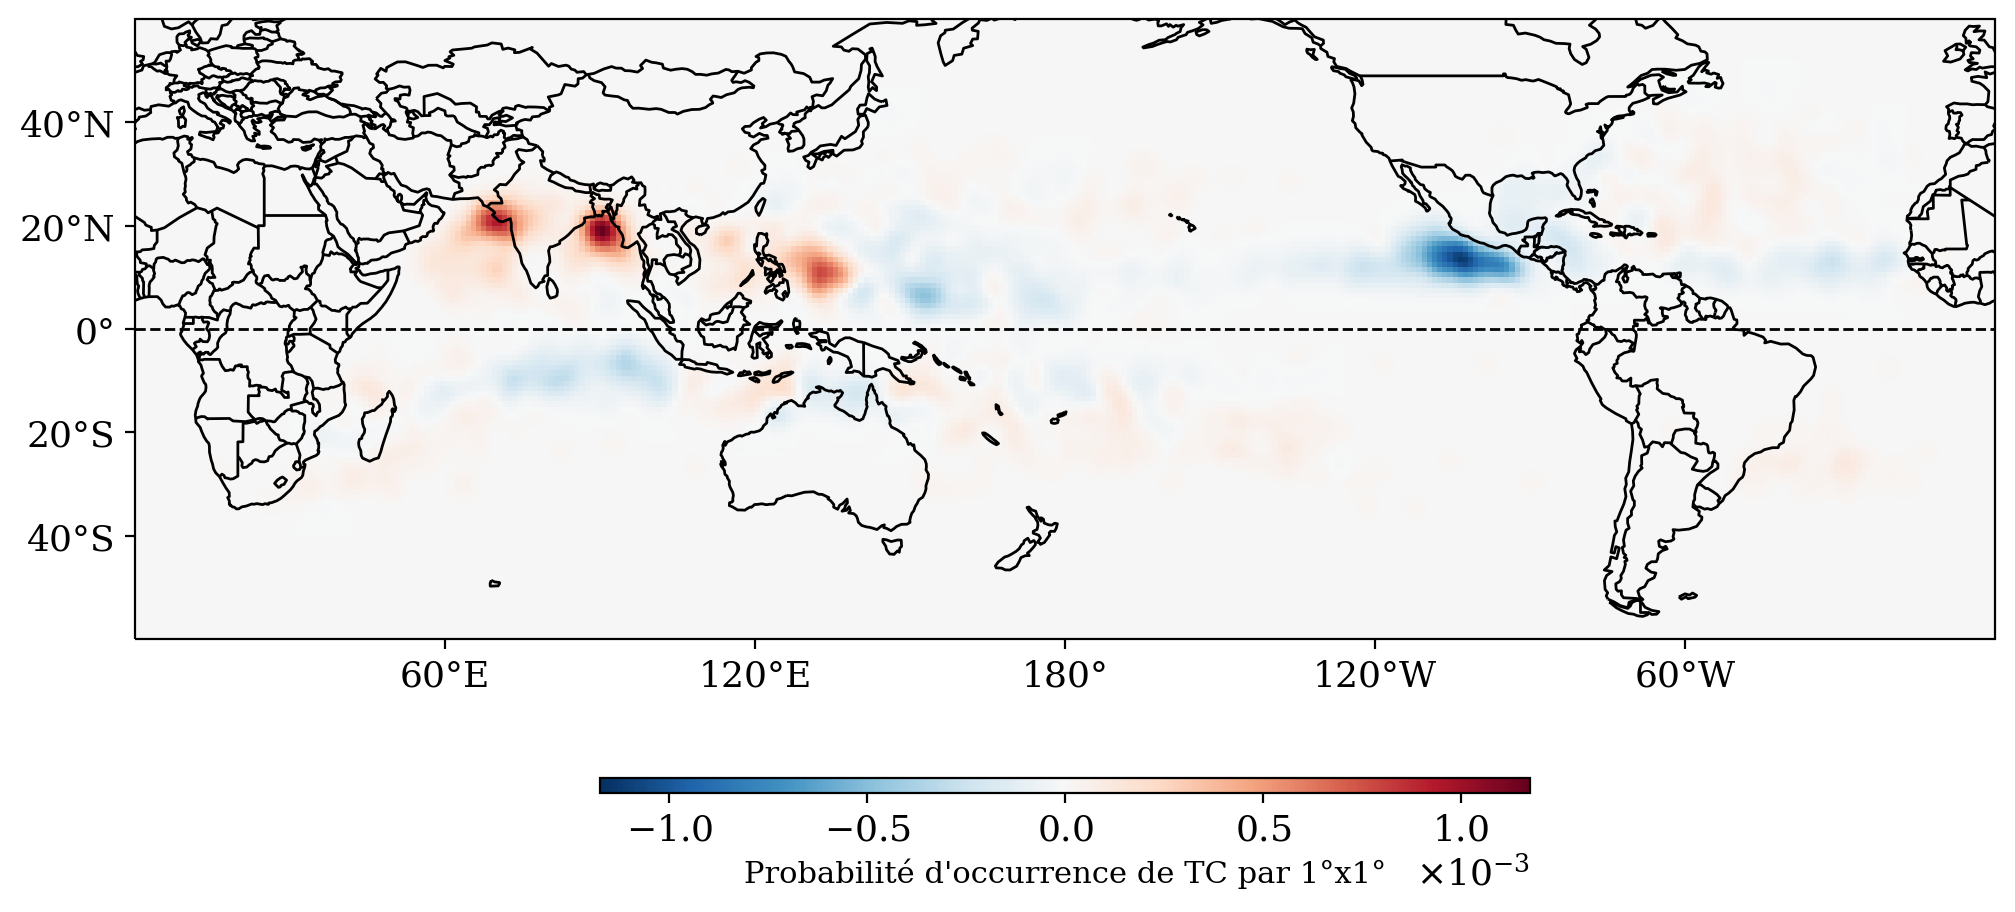
\includegraphics[width=\textwidth]{density_arpege_ibtracs.png}
    \caption{Carte de la différence entre les densités de cyclogénèses moyennes et normalisées ---~lissées au préalable avec un filtre gaussien à \ang{1}
    d'écart-type~--- de la simulation ARPEGE forcée et IBTrACS entre \num{1980} et \num{2010}.}
    \label{fig:density_arpege_ibtracs}
\end{figure}

%La \cref{fig:STJ_PRE625REFT359x} présente quant à elle les moyennes saisonnières de la latitude diagnostiquée par le filtre du STJ pour les deux hémisphères.
%Les variations saisonnières du STJ de la \cref{fig:STJ_PRE625REFT359x} illustrent le caractère dynamique du filtre du STJ, par rapport à une limite en latitude
%fixe. Cette figure met aussi en évidence le caractère saisonnier du filtre, avec un décalage vers les pôles durant les saisons chaudes, et un déport vers
%l'équateur durant la saison froide, les deux étant bien entendu en opposition de phase dans chacun des hémisphères. Cette propriété du seuil dynamique en
%latitude avait déjà été mise en évidence pour le filtre du gradient de géopotentiel à \hPa{200} présenté dans la \cref{sec:filtrage_mid_latitudes}
%(\cref{chap:chapitre_2}), mais n'avait pas été documentée pour le filtre du STJ.

%\begin{figure}[tp]
%    \centering
%    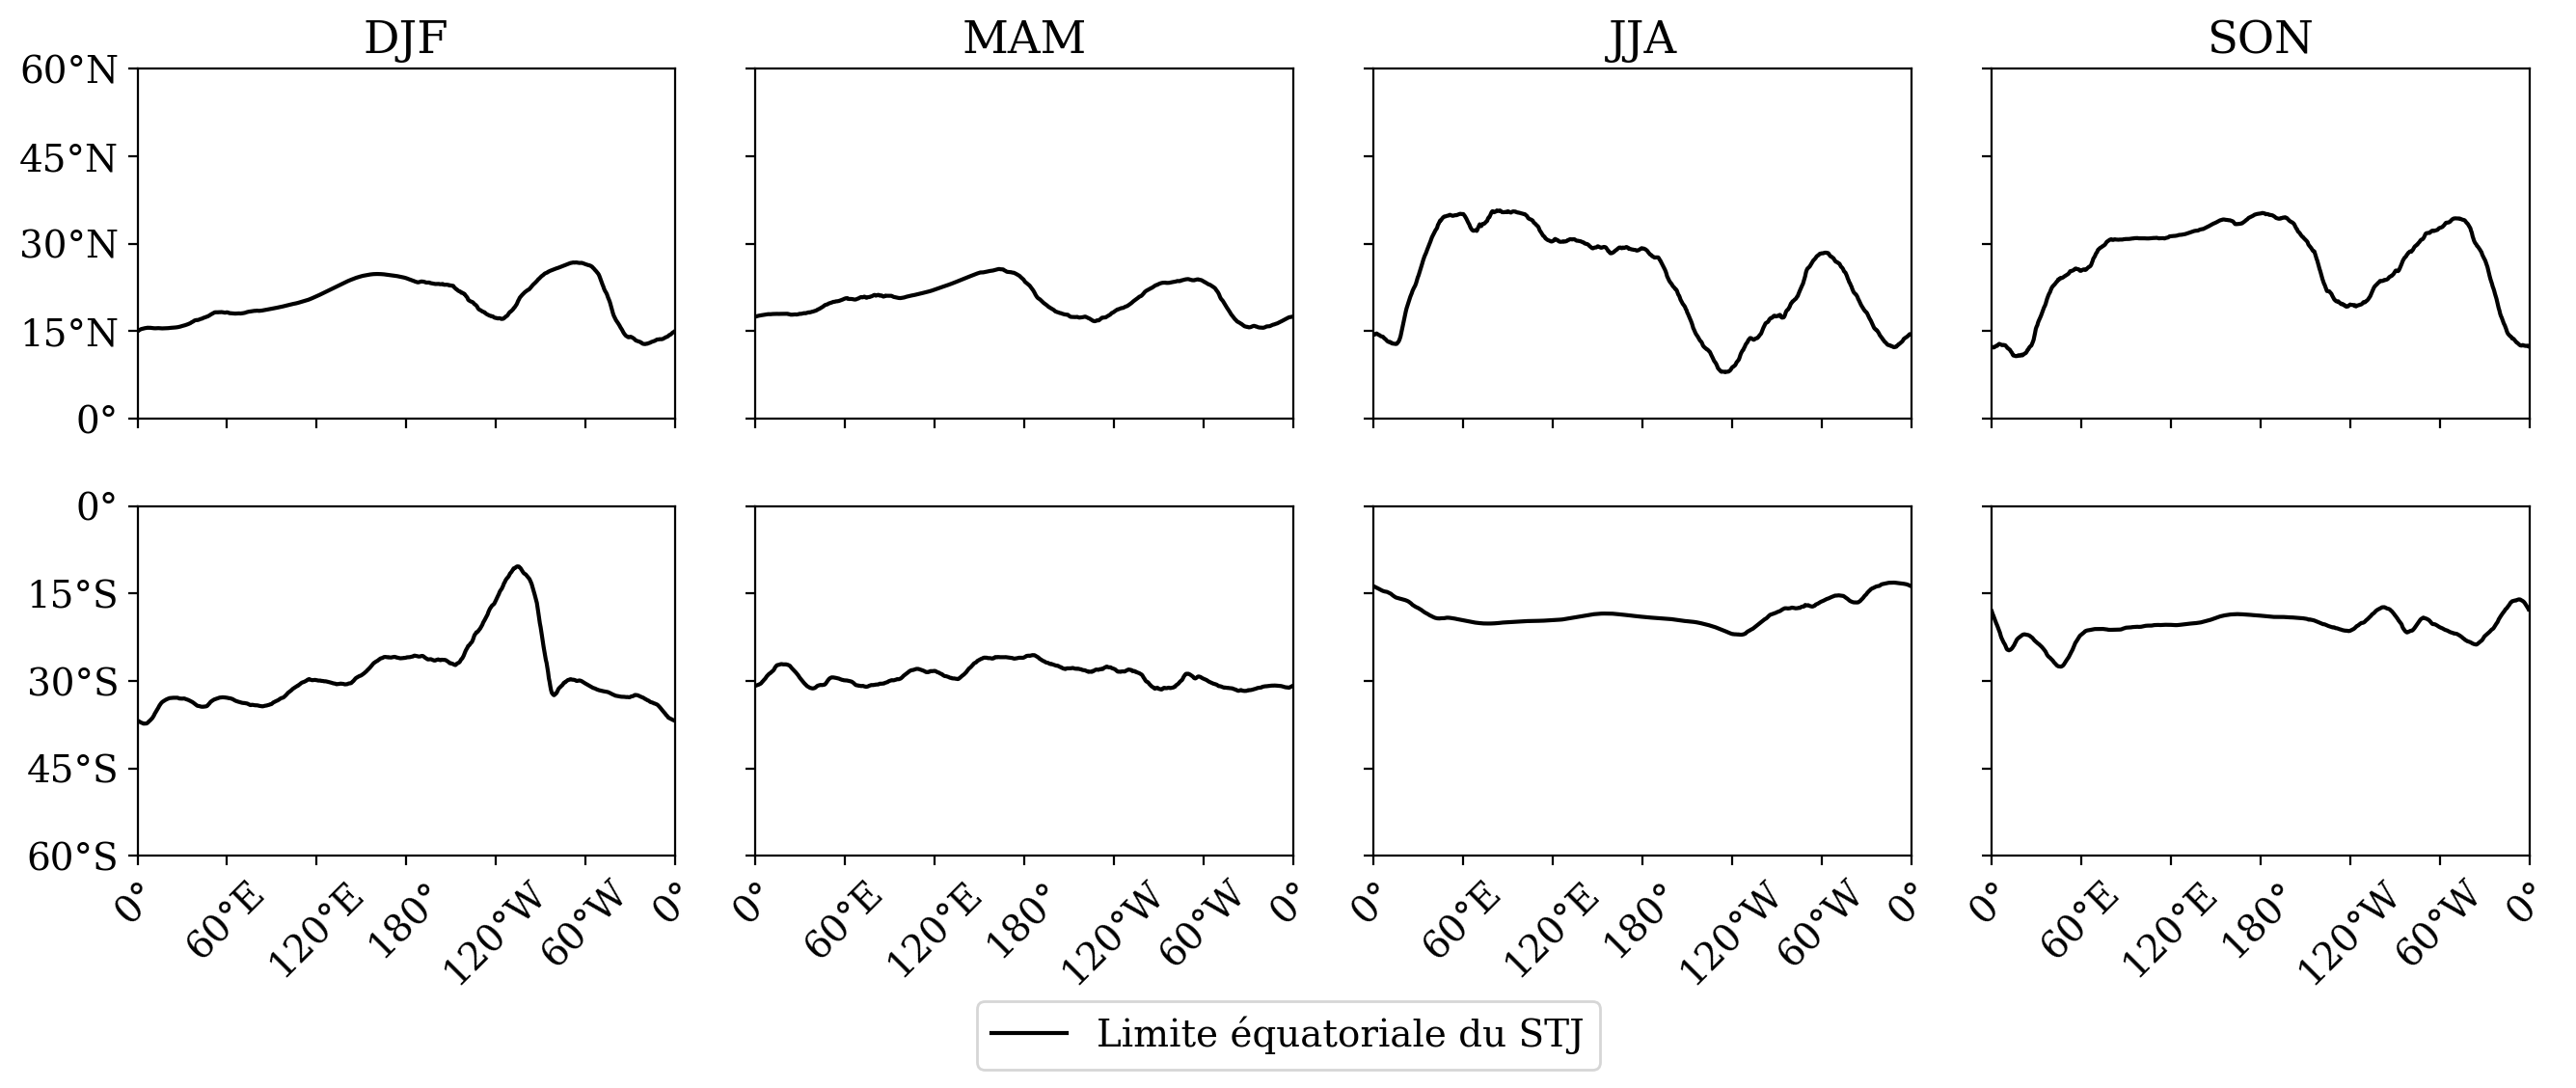
\includegraphics[width=\textwidth]{STJ_season_PRE625REFT359x.png}
%    \caption{Moyennes saisonnières de la latitude de la limite équatoriale du jet subtropical dans la simulation ARPEGE-Climat forcée par HadISST1. Chacune des
%    quatre colonnes correspond à une saison. La première ligne présente le diagnostique pour l'hémisphère nord, tandis que la seconde ligne le présente pour
%    l'hémisphère sud.}
%    \label{fig:STJ_PRE625REFT359x}
%\end{figure}

\subsubsection{Diagnostique ENSO}\label{sec:diag_enso}

Le mode de variabilité El Niño (respectivement La Niña) est caractérisé par une anomalie chaude (respectivement froide) de SST dans l'oćean Pacifique central.
Il existe plusieurs façons de diagnostiquer ce phénomène et qui se distinguent entre elles par la région, ou boîte, utilisée pour calculer l'anomalie de
température, ainsi que par le lissage temporel utilisé. Ces boîtes sont au nombre de \num{4}, réparties entre les côtes de l'Amérique centrale et les îles
Salomon. L'anomalie de SST prise dans une de ces boîtes définit alors un indice El Niño. Ici, nous utilisons l'indice ENSO utilisé pour les besoins
opérationnels de la NOAA, nommé ONI (\textit{Oceanic Niño Index}). L'ONI est défini sur la boîte 3.4, c'est à dire à cheval sur les boîtes \num{3} et \num{4}
(non montrées) et définie entre \ang{120}W et \ang{170}W, et entre \ang{5}S et \ang{5}N. Les anomalies sont lissées sur \num{3} mois glissants, et la référence
climatologique est prise comme la SST moyenne sur toute la période disponible. La \cref{fig:ONI} présente la boîte 3.4 utilisée pour calculer l'anomalie de
température, ainsi que la série temporelle de l'ONI entre janvier \num{1980} et décembre \num{2010}.

\begin{figure}[htpb]
    \centering
    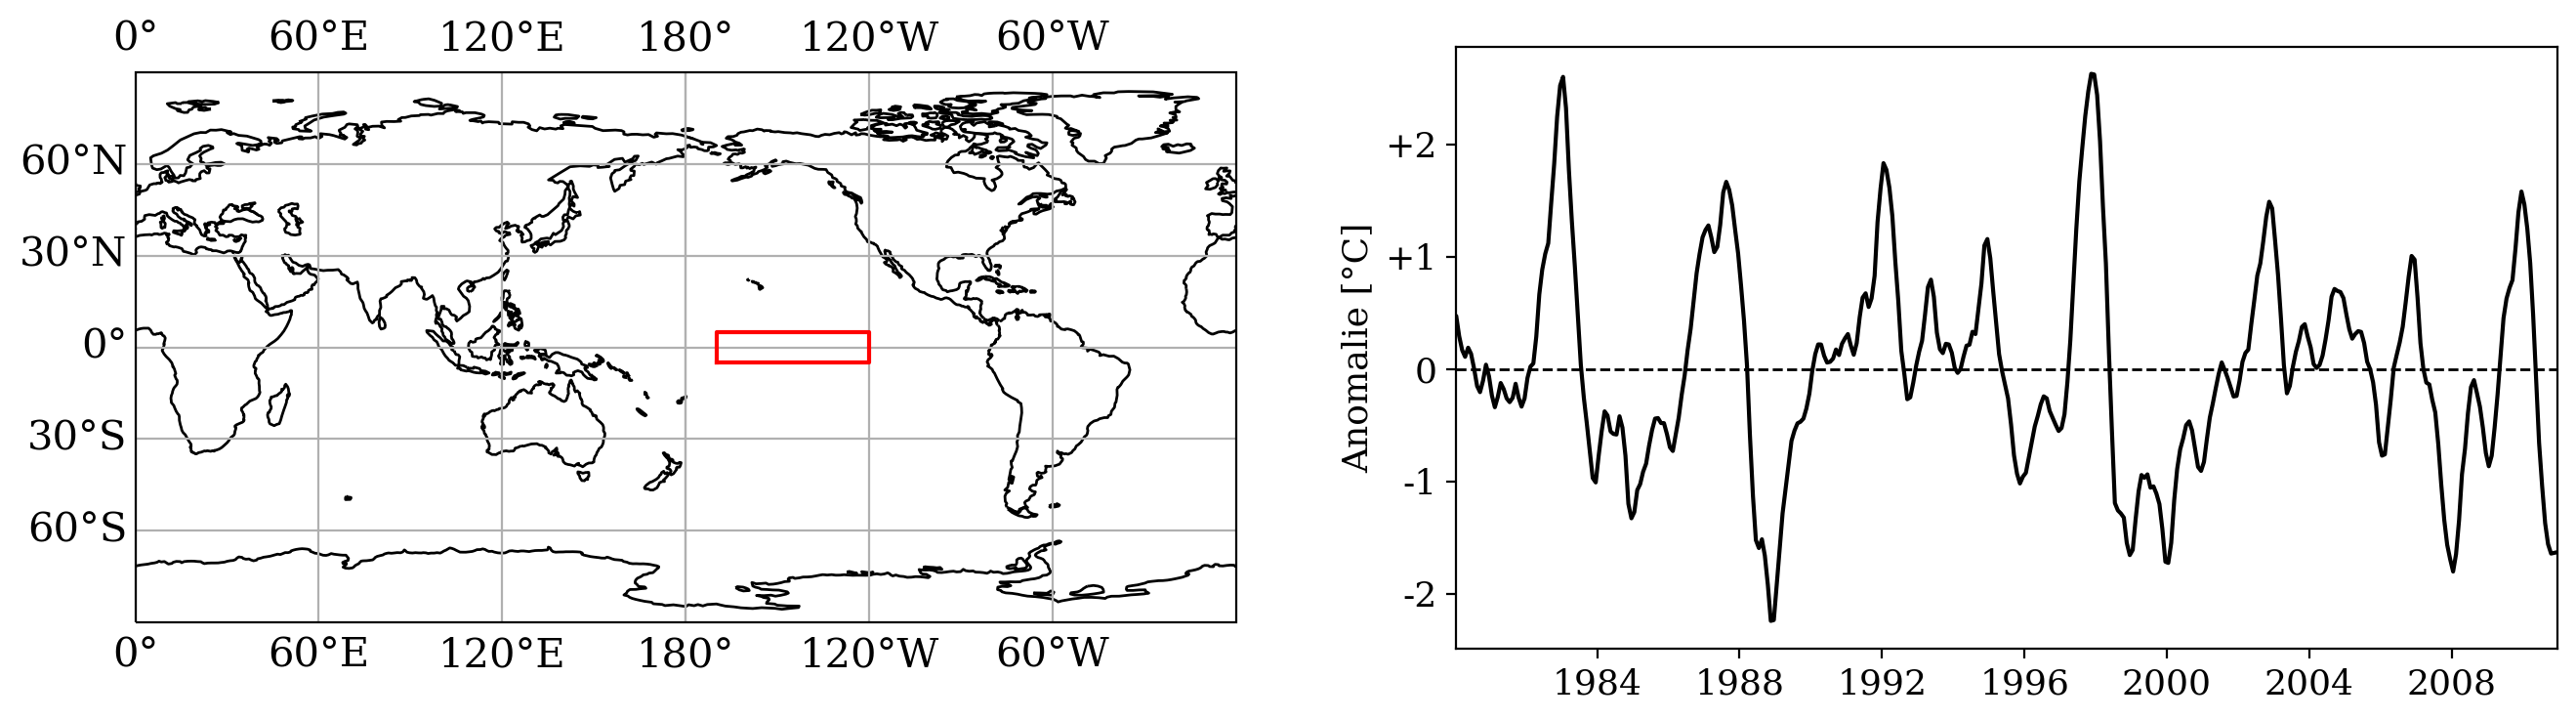
\includegraphics[width=\textwidth]{ONI.png}
    \caption{Boîte 3.4 utilisée pour le calcul de l'ONI (gauche) et série temporelle de l'ONI (droite) évaluée sur la SST mensuelle de la
    simulation ARPEGE forcée par HadISST1.}
    \label{fig:ONI}
\end{figure}

Pour utiliser l'ONI comme prédicteur dans une régression de Poisson, il est nécessaire de le transformer en vecteur de la même taille $m$ (c.f
\cref{chap:chapitre_3}, \cref{sec:regression_poisson}) que les champs spatio-temporels de grande échelle. L'ONI étant, pour un mois donné, un scalaire ; sa
valeur est répliquée en tout point de la grille spatiale souhaitée. Cela revient à considérer que chaque point de l'espace a connaissance à chaque
pas de temps de l'anomalie de SST dans la boîte 3.4.

\subsection{Lien entre ENSO et l'activité cyclonique dans ARPEGE}\label{sec:lien_enso_tracking}

Le lien entre ENSO et l'activité cyclonique tropicale dans les observations et dans les modèles est largement documenté
\parencite{chan_tropical_1985,wu_gcm_1992,landsea_ninosouthern_2000,mcdonald_tropical_2005,lin_enso_2020}. Une phase positive de l'oscillation El-Niño tend à
augmenter la fréquence d'occurence des TC dans certains bassins, notamment dans le Pacifique, et tend à la réduire dans l'océan Indien, et vice versa. Dans
l'Atlantique nord, l'activité cyclonique est traditionnellement anti-corrélée à ENSO, car ce dernier apporte du cisaillement dans l'océan Atlantique. Cependant,
pour déterminer dans quelle mesure l'ajout de l'ONI comme prédicteur dans une régression établie sur les cyclogénèses détectées dans le modèle ARPEGE peut impacter la
fréquence statistiquement modélisée, il convient de quantifier le lien entre l'ONI et l'activité cyclonique dans notre jeu de données.

La \cref{fig:corr_ONI_pt} présente la carte de corrélation entre le nombre annuel de cyclogénèses pour chaque maille d'une grille régulière de \ang{3} de
résolution et l'ONI, aggrégé annuellement de la même façon. Précisons que, à l'instar de toutes les opérations de calcul de variabilité interannuelle
réalisées jusqu'à maintenant, et notamment dans le \cref{chap:chapitre_3}, la fréquence annuelle est calculée pour les saisons cycloniques. Dans l'hémisphère
sud, le nombre de TC pour une saison donnée est donc évalué entre juillet de l'année précédente et juin de l'année courante. Précisons aussi qu'un masque
terre-mer interpolé sur la grille de \ang{3} de résolution est utilisé pour masquer les cyclogénèses détectées sur terre de la
\cref{fig:track_density_PRE625REFT359x}.

\begin{figure}[tpb]
    \centering
    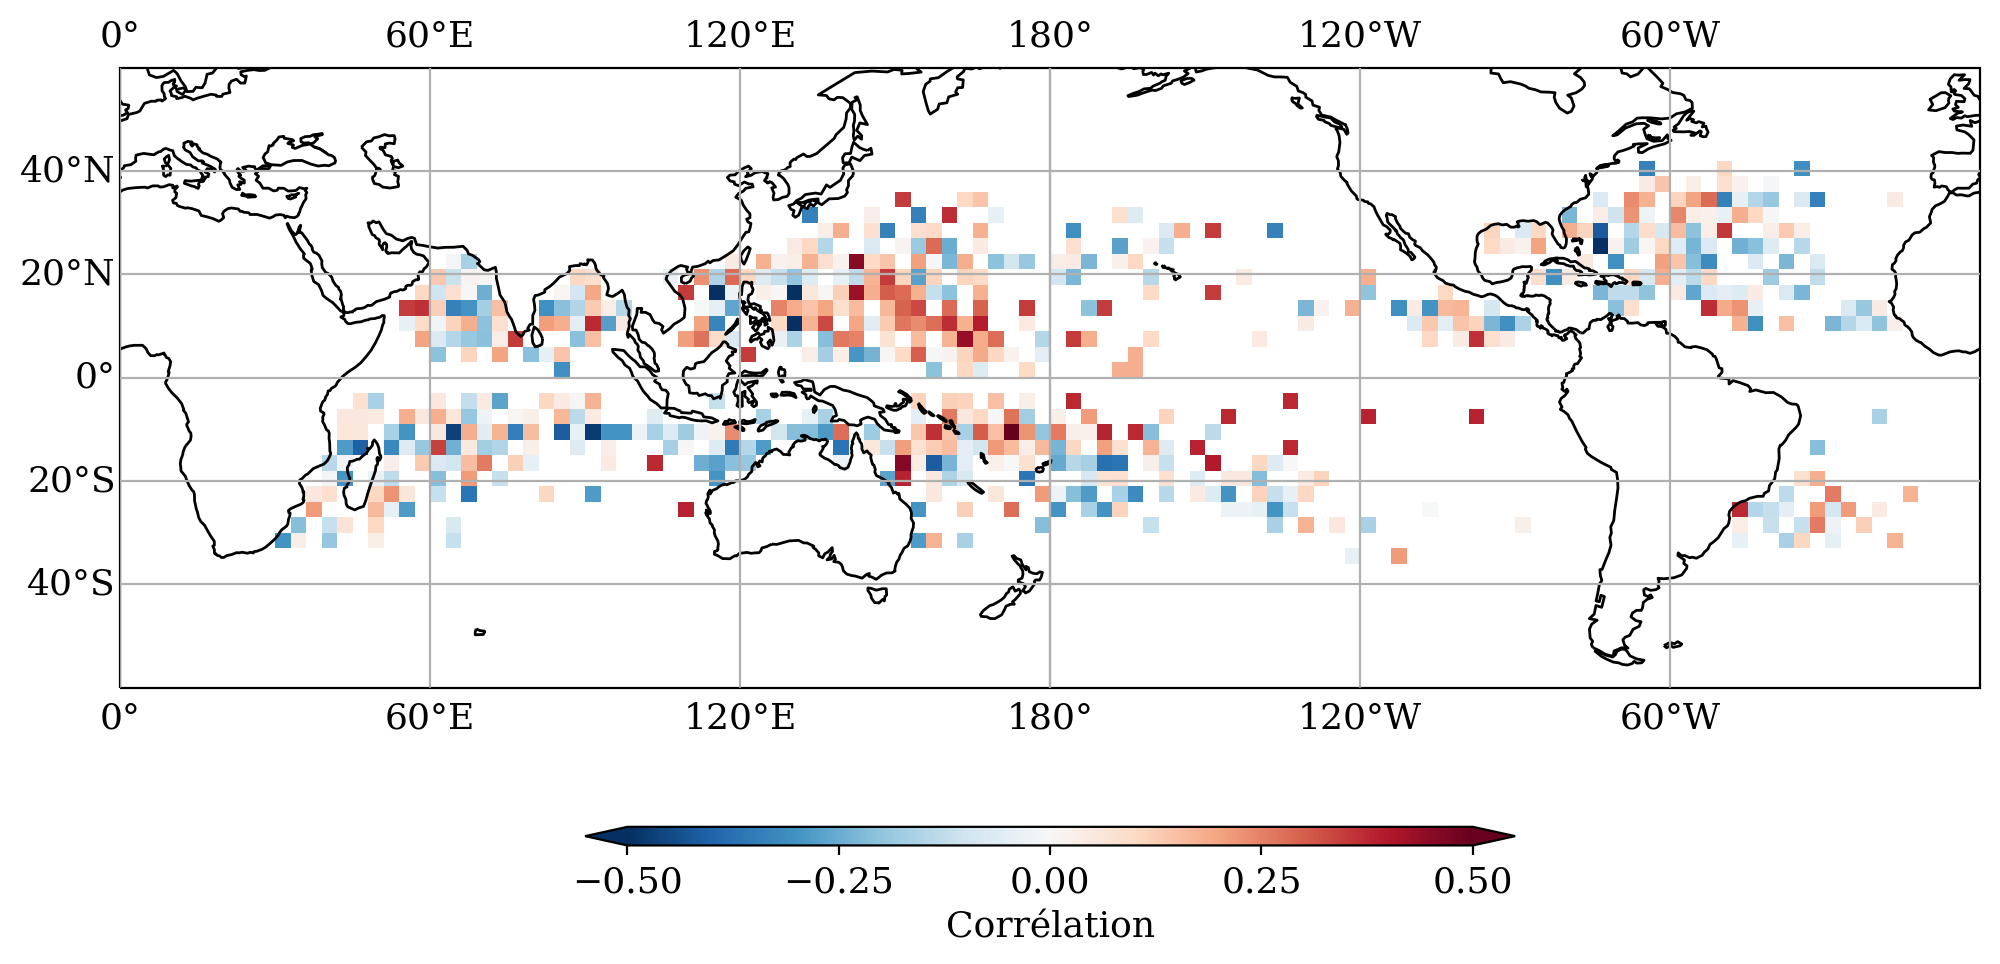
\includegraphics[width=\textwidth]{corr_ONI_tracks.png}
    \caption{Carte de corrélation entre la variabilité interannuelle de l'activité cyclonique par point de grille (\ang{3}x\ang{3}) pour les cyclogénèses
    détectées dans ARPEGE et l'ONI, sur les saisons cycloniques entre \num{1980} et \num{2010}.}
    \label{fig:corr_ONI_pt}
\end{figure}

La \cref{fig:corr_ONI_pt} met en évidence des corrélations contrastées dans les différents bassins d'activité. Le signal le plus clair est noté dans le WPac, à
l'ouest de \ang{180}, avec une corrélation positive dans la plupart des mailles où des cyclogénèses ont été détectées. Certaines dépassent la borne supérieure
de la carte des couleurs fixée à \num{0.5}. Dans le bassin EPac, le peu de cyclogénèses disponibles (voir
\cref{fig:track_density_PRE625REFT359x,fig:density_arpege_ibtracs}) empêche l'interprétation de la corrélation. Dans le SPac, des corrélations positives
relativement fortes sont notées dans la partie nord, tandis que ces dernières s'inversent au delà de \ang{20}S. Dans le bassin SIndE, ENSO apparaît clairement
anti-corrélée à l'activité cyclonique, à l'exception de quelques mailles. Pour les bassins SIndW NInd et NAtl, le signal est plus contrasté mais laisse également
entrevoir dans l'ensemble une possible anti-corrélation.

Pour évaluer le lien entre l'activité cyclonique détectée et la variabilité El Niño dans ces bassins où la \cref{fig:corr_ONI_pt} ne permet pas de dégager une
conclusion nette, la corrélation est évaluée à l'échelle du bassin tout entier. Spécifiquement, les cyclogénèses sont comptabilisées sur la grille d'origine de
la simulation (T359, soit \ang{0.5}), puis l'activité est intégrée spatialement sur les bassins océaniques usuels selon la méthodologie employée dans le
\cref{chap:chapitre_3}. Enfin, la corrélation avec la variabilité interannuelle de l'ONI est évaluée pour chacun des bassins. La
\cref{fig:corr_ONI_bassin} présente les coefficients de corrélation $r$ ainsi que les valeurs-p associées.

\begin{figure}[tpb]
    \centering
    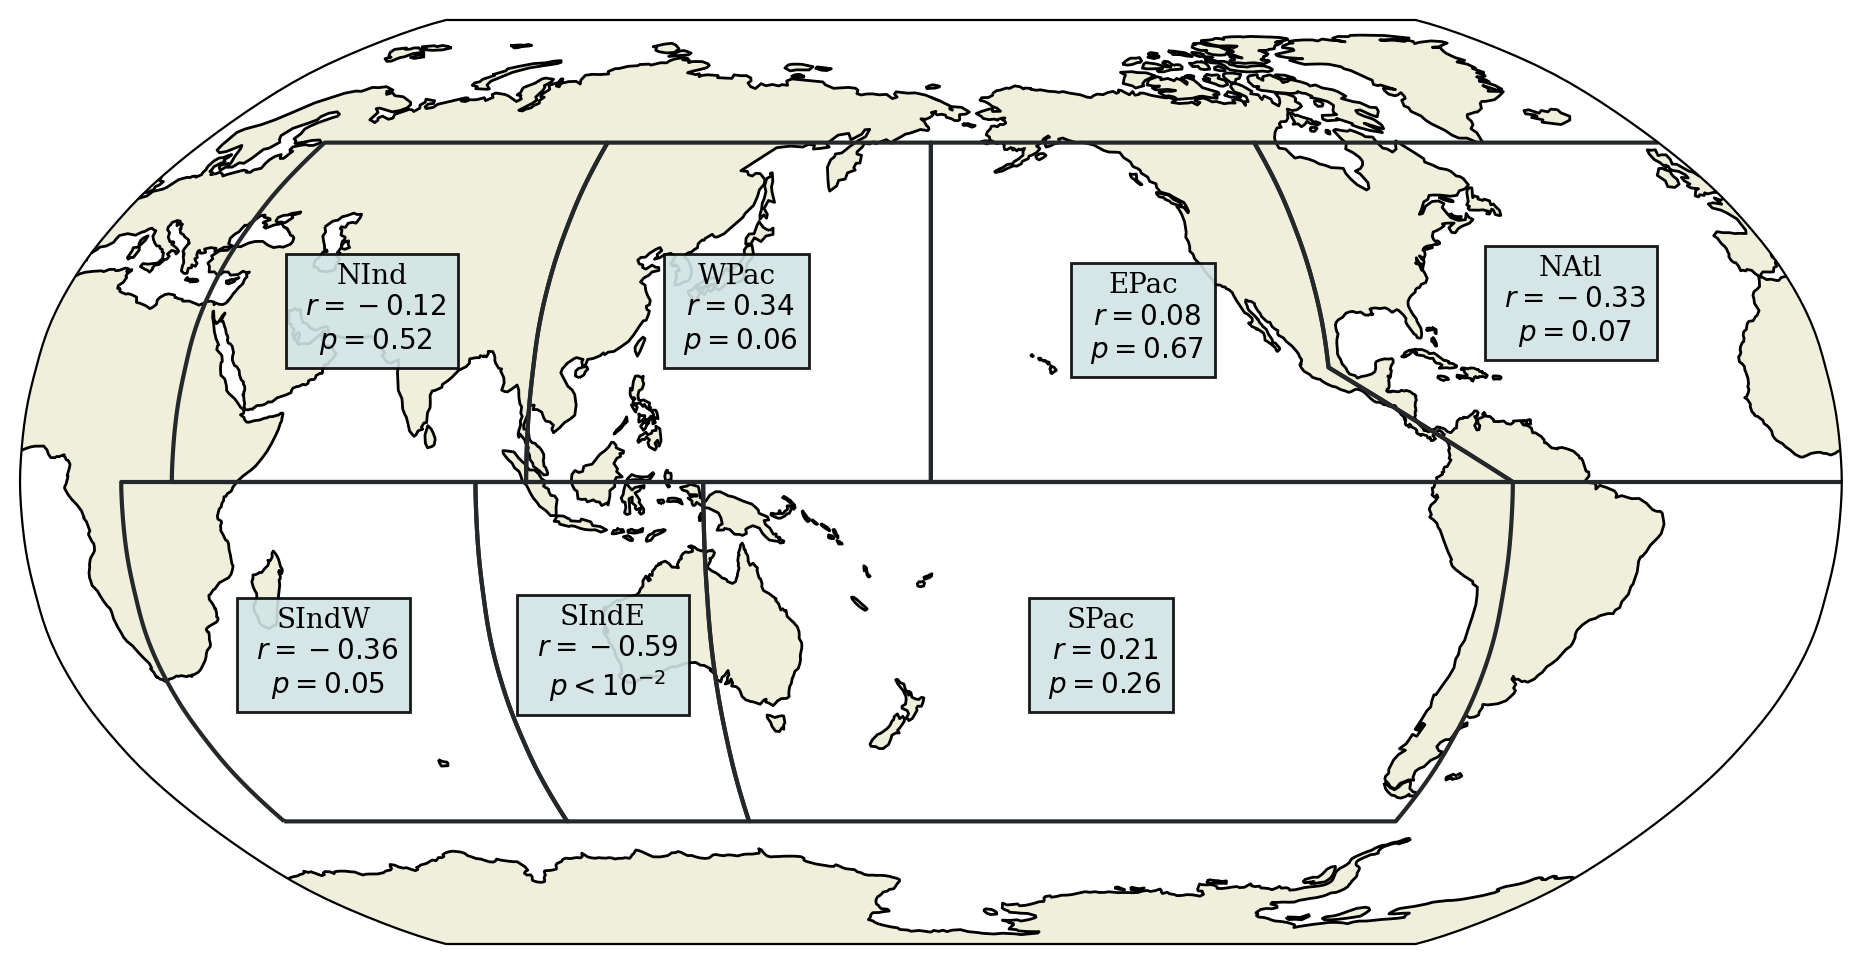
\includegraphics[width=\textwidth]{corr_ONI_bassin}
    \caption{corrélation entre la variabilité interannuelle de l'activité cyclonique détectée dans ARPEGE et l'ONI à l'échelle des bassins océaniques.}
    \label{fig:corr_ONI_bassin}
\end{figure}

Pour les bassins WPac et SIndE, la \cref{fig:corr_ONI_bassin} confirme ce que laisse deviner la \cref{fig:corr_ONI_pt}, à savoir une corrélation dans le
premier, évaluée à \num{0.34} et à la limite de la significativité sous un seuil de \prct{95}, et une anti-corrélation significative dans le second à
\num{-0.59}. La \cref{fig:corr_ONI_bassin} permet également de lever l'ambigüité pour les bassins où le lien est contrasté sur la \cref{fig:corr_ONI_pt}. Ainsi
l'activité cyclonique dans le bassin SIndW est également présenté comme anti-corrélée à l'ONI avec \num{-0.36}, là aussi à la limite de la significativité, et
pareillement dans le bassin NAtl avec \num{-0.33}, bien qu'avec une valeur-p de \num{0.07}. En revanche, le bassin EPac ne présente aucune corrélation, et
celles des bassins NInd et SPac ne sont pas significatives. À titre de référence, cette carte réalisée entre ERA5 et IBTrACS signale une corrélation de
\num{0.54} dans le bassin EPac et de \num{-0.43} dans le bassin NAtl. La corrélation dans le bassin SIndE est inchangée par rapport à celle mesurée ici, mais
les bassins WPac et SIndW sont néanmoins parfaitement décorrélés.

Le lien entre l'activité cyclonique telle que détectée par le schéma de détection du CNRM appliqué au modèle ARPEGE d'une part, et le mode de variabilité El
Niño est dans l'ensemble cohérent. Plusieurs bassins océaniques présentent des corrélations à la limite de la significativité statistique, et c'est par
conséquent dans ces bassins là qu'une éventuelle plus-value de l'ajout de l'ONI comme prédicteur dans une régression de Poisson peut être attendue.

\subsection{Application de la régression}

On applique ici la régression de Poisson selon la même méthodologie employée pour construire l'indice nommé M10 dans la \cref{sec:apport_res_temporel_spatial},
mais appliquée à la simulation ARPEGE. On utilise donc en prédictant les cyclogénèses détectées par le traqueur du CNRM dans la simulation historique ARPEGE
forcée par HadISST1. Ces dernières, de même que les champs de grande échelle utilisés comme prédicteurs, transposées sur une grille régulière de \ang{1} de
résolution et agrégées au pas de temps mensuel. Ici encore, la taille de la matrice $\mathbf{x}$ des prédicteurs est le principal facteur limitant la résolution
spatiale pour réaliser la régression, et est la raison pour laquelle nous n'utilisons pas la grille T359 d'origine. Nous utilisons les mêmes variables
thermiques et dynamiques que pour le TCS et pour les \cref{sec:apport_res_temporel_spatial,sec:indice_regional}, à savoir la vorticité absolue bornée à
\SI{3.7e-5}{\per\second} $\eta$, le cisaillement vertical $V_{\mathrm{shear}}$ entre \hPa{850} et \hPa{200}, l'humidité relative $H$ à \hPa{600} et la SST
relative $T$.

Nous définissons dans un premier temps l'équivalent de l'indice M10 pour ARPEGE, nommé AM10. Nous réalisons ensuite une seconde régression en ajoutant à
ces quatre variables décrivant l'environnement de grande échelle le champ artificiel de l'ONI, défini en tout point de la grille comme l'anomalie
mensuelle de SST dans la boîte 3.4 présentée dans la \cref{sec:diag_enso}. L'indice incluant l'ONI comme prédicteur est nommé OAM10, abrégé en OA. La régression
avec l'ONI comme prédicteur est appliquée aussi bien à l'échelle globale qu'à l'échelle des bassins individuels. Dans le second cas, la méthodologie employée
dans la \cref{sec:indice_regional} pour construire l'indice LM10 est transposée aux prédicteurs et prédictant ARPEGE, notamment pour ce qui concerne la
calibration de l'indice régional sur la fréquence annuelle moyenne inférée par son homologue global. L'indice régional est alors nommé LOAM10, ou simplement
LOA, puisqu'il est entendu que, contrairement au \cref{chap:chapitre_3}, les régressions sont uniquement faites avec les moyennes mensuelles à \ang{1} de
résolution.

Enfin, précisons que les cyclogénèses détectées sur terre sont masquées, si bien que la fréquence annuelle de référence pour la calibration des indices globaux
est réduite à \num{52.32} TC par an. Bien que ce nombre soit bien différent de la fréquence de référence issue IBTrACS utilisée dans le \cref{chap:chapitre_3},
cela n'a aucune importance dès lors que tous les indices sont calibrés sur cette valeur. Le TCS de \textcite{tippett_poisson_2011} est également pris comme
référence pour la comparaison des résultats.

\subsubsection{Régressions globales}

Nous nous intéressons dans un premier temps aux coefficients obtenus pour les régressions globales AM10 et OAM10. L'indice de cyclogénèse AM10 est donné
ci-dessous :
%
\begin{align*}
\tag{AM10}
    \mu &= \exp \big( b_0 + b_\eta \eta + b_{V_{\mathrm{shear}}} V_{\mathrm{shear}} + b_H H + b_T T + \log \cos \phi \big)\\
        &= \exp \big( \num{-18.6861} + \num{2.4363} \eta - \num{0.0192} V_{\mathrm{shear}} + \num{0.0454} H + \num{0.4202} T + \log \cos \phi \big)
\end{align*}
%
Les coefficients de AM10 sont à mettre en regard avec ceux obtenus pour l'indice M10, obtenus entre ERA5 et IBTrACS dans le \cref{chap:chapitre_3}. Ces derniers
peuvent être consultés dans le \cref{tab:fit_spatial_temporel}, \vpageref{tab:fit_spatial_temporel}. Le coefficient $b_H$ est réduit d'environ \num{0.072} à
\num{0.045}, soit une valeur proche du coefficient associé à l'humidité relative du TCS (\num{0.05}). Les coefficients $b_T$ sont quant à eux quasi identiques,
à \num{0.01} près. Cela peut vraisemblablement s'expliquer par le fait que la réanalyse ERA5 assimile des données la SST issue de la base de données HadISST2
jusqu'en \num{2007}. La sensibilité au cisaillement vertical est néanmoins réduite dans AM10, passant d'environ \num{-0.1} dans ERA5 à environ \num{-0.02} dans
ARPEGE, soit une sensibilité cinq fois moindre dans le modèle de climat. Cette valeur du coefficient apparaît néanmoins comme statistiquement significative
(ainsi que tous les autres coefficients) en dépit de sa valeur proche de \num{0}. La régression indique en effet des pourcentiles \prct{2.5} et \prct{97.5} de
respectivement \num{-0.027} et \num{-0.011} pour $b_{V_{\mathrm{shear}}}$, et une valeur-p inférieure à \num{1e-3}. Le coefficient associé à la vorticité
absolue est celui présentant la plus grande différence pasant d'environ \num{1.40} pour M10 à \num{2.44} pour AM10. Une valeur si élévée de $b_\eta$ est
cohérente avec le biais septentrional dans les cyclogénèses détectées dans ARPEGE (voir \cref{fig:density_arpege_ibtracs}), puisqu'il a été largement montré
dans le \cref{chap:chapitre_3} que des valeurs élevées de ce paramètre sont associées à une activité simulée par la régression plus éloignée de l'équateur.

La relation pour l'indice OA est donnée ci-dessous :
%
\begin{align*}
    \tag{OA}
    \mu &= \exp \big( b_0 + b_\eta \eta + b_{V_{\mathrm{shear}}} V_{\mathrm{shear}} + b_H H + b_T T + b_{\mathrm{ONI}} \mathrm{ONI} + \log \cos \phi \big)\\
        &= \begin{aligned}[t]\exp \big( \num{-18.7099} + \num{2.4430}\, \eta - \num{0.0192}\, V_{\mathrm{shear}} \,+\, &\num{0.0454}\, H + \num{0.4221}\, T + \\&\underbrace{\num{0.0638}\, \mathrm{ONI}}_{\mathrm{Indice\ ENSO}} + \log \cos \phi \big)\end{aligned} \end{align*}
%
L'ajout de l'ONI dans la régression ne modifie que très marginalement les coefficients associés aux autres prédicteurs. On ne note qu'une très légère hausse de
$b_\eta$ ainsi qu'une augmentation toute aussi faible de $b_T$. La régression indique cependant une sensibilité positive à l'ONI avec une valeur
$b_{\mathrm{ONI}}$ d'environ \num{0.06}. Cela signifie qu'à l'échelle globale, un changement de $+$\SI{1}{\degreeCelsius} de l'anomalie de SST dans la région
3.4 provoque une hausse de la fréquence d'occurrence modélisée par la régression de l'ordre \prct{6}. Cette valeur apparaît comme statistiquement significative,
avec une valeur-p de \num{0.024}. Il s'agit toutefois de la valeur-p la plus élevée notée jusqu'à maintenant, ces dernières étant sinon systématiquement
inférieures à \num{1e-3}, pour toutes les régressions réalisées dans le \cref{chap:chapitre_3} et dans le chapitre présent. La régression indique un AIC
\parencite[\textit{Akaike Information Criterion},][]{akaike_information_1998} ---~c'est à dire une log-vraisemblance ajustée par le nombre de prédicteurs~---
légèrement réduite par rapport à AM10, passant en effet de \num{24752} à \num{24747}, indiquant une régression de qualité légèrement supérieure lorsque la
variable ONI est introduite.

Néanmoins, la \cref{sec:lien_enso_tracking} montre que le lien entre ENSO et l'activité cyclonique n'est pas uniforme dans l'espace, avec certaines régions
exprimant une corrélation positive, et d'autres une anti-corrélation. Un indice de cyclogénèse formulé sur l'ONI et dont la régression est menée à l'échelle
globale ne peut donc satisfaire le rapport entre ce mode de variabilité et l'activité constatée dans tous les bassins. Sachant cela, il est permis de penser que
le signe positif de $b_{\mathrm{ONI}}$ pour AM10 et sa significativité statistique sont fortement influencés par le bassin WPac, présentant sur la
\cref{fig:corr_ONI_bassin} une corrélation positive, et influençant d'avantage la régression en sa qualité de bassin le plus actif. C'est pour cette raison que la
régression est répétée à l'échelle des bassins.

\subsubsection{Régressions locales}

Le \cref{tab:coefs_LOA} présente les coefficients obtenus pour chacune des régressions faites à l'échelle des bassins océaniques. On s'intéresse tout
particulièrement aux coefficients associés à l'ONI, aux intervalles de confiance ainsi qu'à la significativité de l'ajout de ce prédicteur dans l'indice LOA.

\begin{table}[htpb]
    \centering
    \caption{Coefficients estimés des prédicteurs pour les régressions réalisées à l'échelle des bassins océaniques avec l'ONI. Les pourcentiles \prct{2.5},
    \prct{97.5} des valeurs de $b_{\mathrm{ONI}}$ sont données, de même que la valeur-p pour ce coefficient. La colonne Fréquence indique le nombre de TC par an
    dans chacun des bassins. Chaque indice régional est calibré sur la fréquence annuelle moyenne de l'indice OA pour ce bassin.}
    \label{tab:coefs_LOA}
    \resizebox{\textwidth}{!}{
    \begin{tabular}{lrrrrrrrrrr}
       \toprule\toprule 
       \multicolumn{1}{c}{Bassin} & \multicolumn{6}{c}{Coefficients} & \multicolumn{3}{c}{ONI} & \multicolumn{1}{c}{Fréquence}\\
       \midrule
                                  & $b_0$ & $b_{\eta}$ & $b_{V_{\mathrm{shear}}}$ & $b_H$ & $b_T$ & $b_{\mathrm{ONI}}$ & \prct{2.5} & \prct{97.5} & valeur-p \\
       \midrule
       NAtl    & \num{-16.7188} & \num{2.3260} & \num{-0.0467} & \num{0.0219} & \num{0.3147} & \num{-0.0737} & \num{-0.237} & \num{0.089} & \num{0.376} & \num{6.41} \\
       WPac    & \num{-17.2232} & \num{1.9807} & \num{-0.0321} & \num{0.0501} & \num{0.3457} & \num{0.2184} & \num{0.116} & \num{0.321} & $< 10^{-3}$ & \num{19.40} \\
       EPac    & \num{-16.9821} & \num{2.0161} & \num{-0.0434} & \num{0.0352} & \num{0.3874} & \num{0.0790} & \num{-0.192} & \num{0.350} & \num{0.568} & \num{5.54} \\
       NInd    & \num{-19.9302} & \num{2.8346} & \num{-0.0450} & \num{0.0624} & \num{0.2984} & \num{0.0559} & \num{-0.081} & \num{0.193} & \num{0.425} & \num{3.98} \\
       SPac    & \num{-19.5598} & \num{2.8841} & \num{-0.0397} & \num{0.0340} & \num{0.4375} & \num{0.1797} & \num{0.053} & \num{0.306} & \num{0.005} & \num{10.12} \\ 
       SIndW   & \num{-17.8103} & \num{2.4274} & \num{-0.0367} & \num{0.0385} & \num{0.3672} & \num{-0.1257} & \num{-0.281} & \num{0.030} & \num{0.113} & \num{3.96} \\
       SIndE   & \num{-19.3702} & \num{3.0105} & \num{-0.1024} & \num{0.0403} & \num{0.4964} & \num{-0.1164} & \num{-0.304} & \num{0.071} & \num{0.224} & \num{2.09} \\
       \bottomrule
    \end{tabular}
    }
\end{table}

Les bassins NInd et EPac présentent les valeurs-p associées à leur coefficient $b_{\mathrm{ONI}}$ les plus élevées de toutes, jusqu'à \num{0.568} pour ce
dernier. Ces mêmes bassins présentaient également les liens les moins prononcés entre ENSO et la variabilité interannuelle dans la
\cref{sec:lien_enso_tracking}. Dans le bassin NAtl, la variable ONI apparait non-significative avec une valeur-p de \num{0.376}. Le coefficient
$b_{\mathrm{ONI}}$, valant environ \num{-0.07}, reflète toutefois le signe du coefficient de corrélation de la \cref{fig:corr_ONI_bassin}, et l'intervalle de
confiance ---~bien que traversant le \num{0}~--- est clairement plus situé du côté des valeurs négatives que des valeurs positives, avec des quantiles
\num{0.025} et \num{0.975} de respectivement \num{-0.237} et \num{0.089}. Un constat similaire peut être fait pour les bassins SIndW et SIndE. Les valeurs-p y
sont en effet supérieures à \num{0.05}, mais leurs coefficients, de respectivement \num{-0.13} et \num{-0.12}, de même que leur intervalle de confiance exprimé
par les pourcentiles \prct{2.5} et \prct{97.5}, sont cohérents avec les résultats de la \cref{fig:corr_ONI_bassin}. Notons que des deux bassins, le SIndW
présente la valeur-p la plus faible à \num{0.113}. Enfin, les régressions faites dans les bassins SPac et WPac acceptent toutes deux le prédicteur ONI, avec une
valeur-p $\leq$ \num{0.05}, bien que le premier soit en limite de significativité. Le coefficient $b_{\mathrm{ONI}}$ dans le bassin WPac est par ailleurs le
plus élevé de tous avec \num{0.22}. Cela conforte la suspicion selon laquelle ce bassin influence fortement le signe du coefficient dans l'indice global OA. Il
convient de noter que la significativité dans le bassin SPac d'une part, et la non-significativité dans les bassins SIndW et SIndE n'étaient pas nécessairement
attendues, puisque la \cref{fig:corr_ONI_bassin} fournit l'information inverse. 

Ainsi, les valeurs prises dans les différentes régions par le coefficient $b_{\mathrm{ONI}}$ reflètent, au moins par leur signe, le lien présenté entre la
variabilité El Niño et l'activité cyclonique détectée dans la simulation ARPEGE forcée, en dépit d'une significativité peu franche, à l'exception notable du
bassin WPac. L'alternance entre le signe du coefficient justifie néanmoins la construction d'indices régionaux plutôt que globaux pour l'ajout de prédicteurs
dont l'effet sur l'activité cyclonique n'est pas uniforme dans toutes les régions du monde.

\subsubsection{Variabilité interannuelle}

La \cref{fig:variability_ONI} présente les variations du nombre de TC d'une saison cyclonique à l'autre pour les trois indices établis sur la simulation ARPEGE
historique, pour le TCS ainsi que les variations vues par le schéma de détection du CNRM, pour les sept bassins définis sur la \cref{fig:corr_ONI_bassin}. Le
bassin NInd est en effet inclus dans l'analyse puisque la détection objective de TC dans la simulation permet d'avoir une série complète, contrairement à
IBTrACS dans le \cref{chap:chapitre_3}. Rappelons que, à l'instar de la \cref{sec:indice_regional} du \cref{chap:chapitre_3}, l'indice LOA est en fait défini
par un indice régional différent pour chaque bassin, dont les coefficients sont donnés dans le \cref{tab:coefs_LOA}. La variabilité temporelle du nombre de TC
détectés dans ARPEGE par le traqueur du CNRM est noté \textquote{Tracks}. La significativité statistique de la corrélation entre les séries temporelles des
quatre indices avec les tracks pour chacun des sept bassins est présenté dans le \cref{tab:pvalues_ONI}.

\begin{figure}[p]
    \centering
    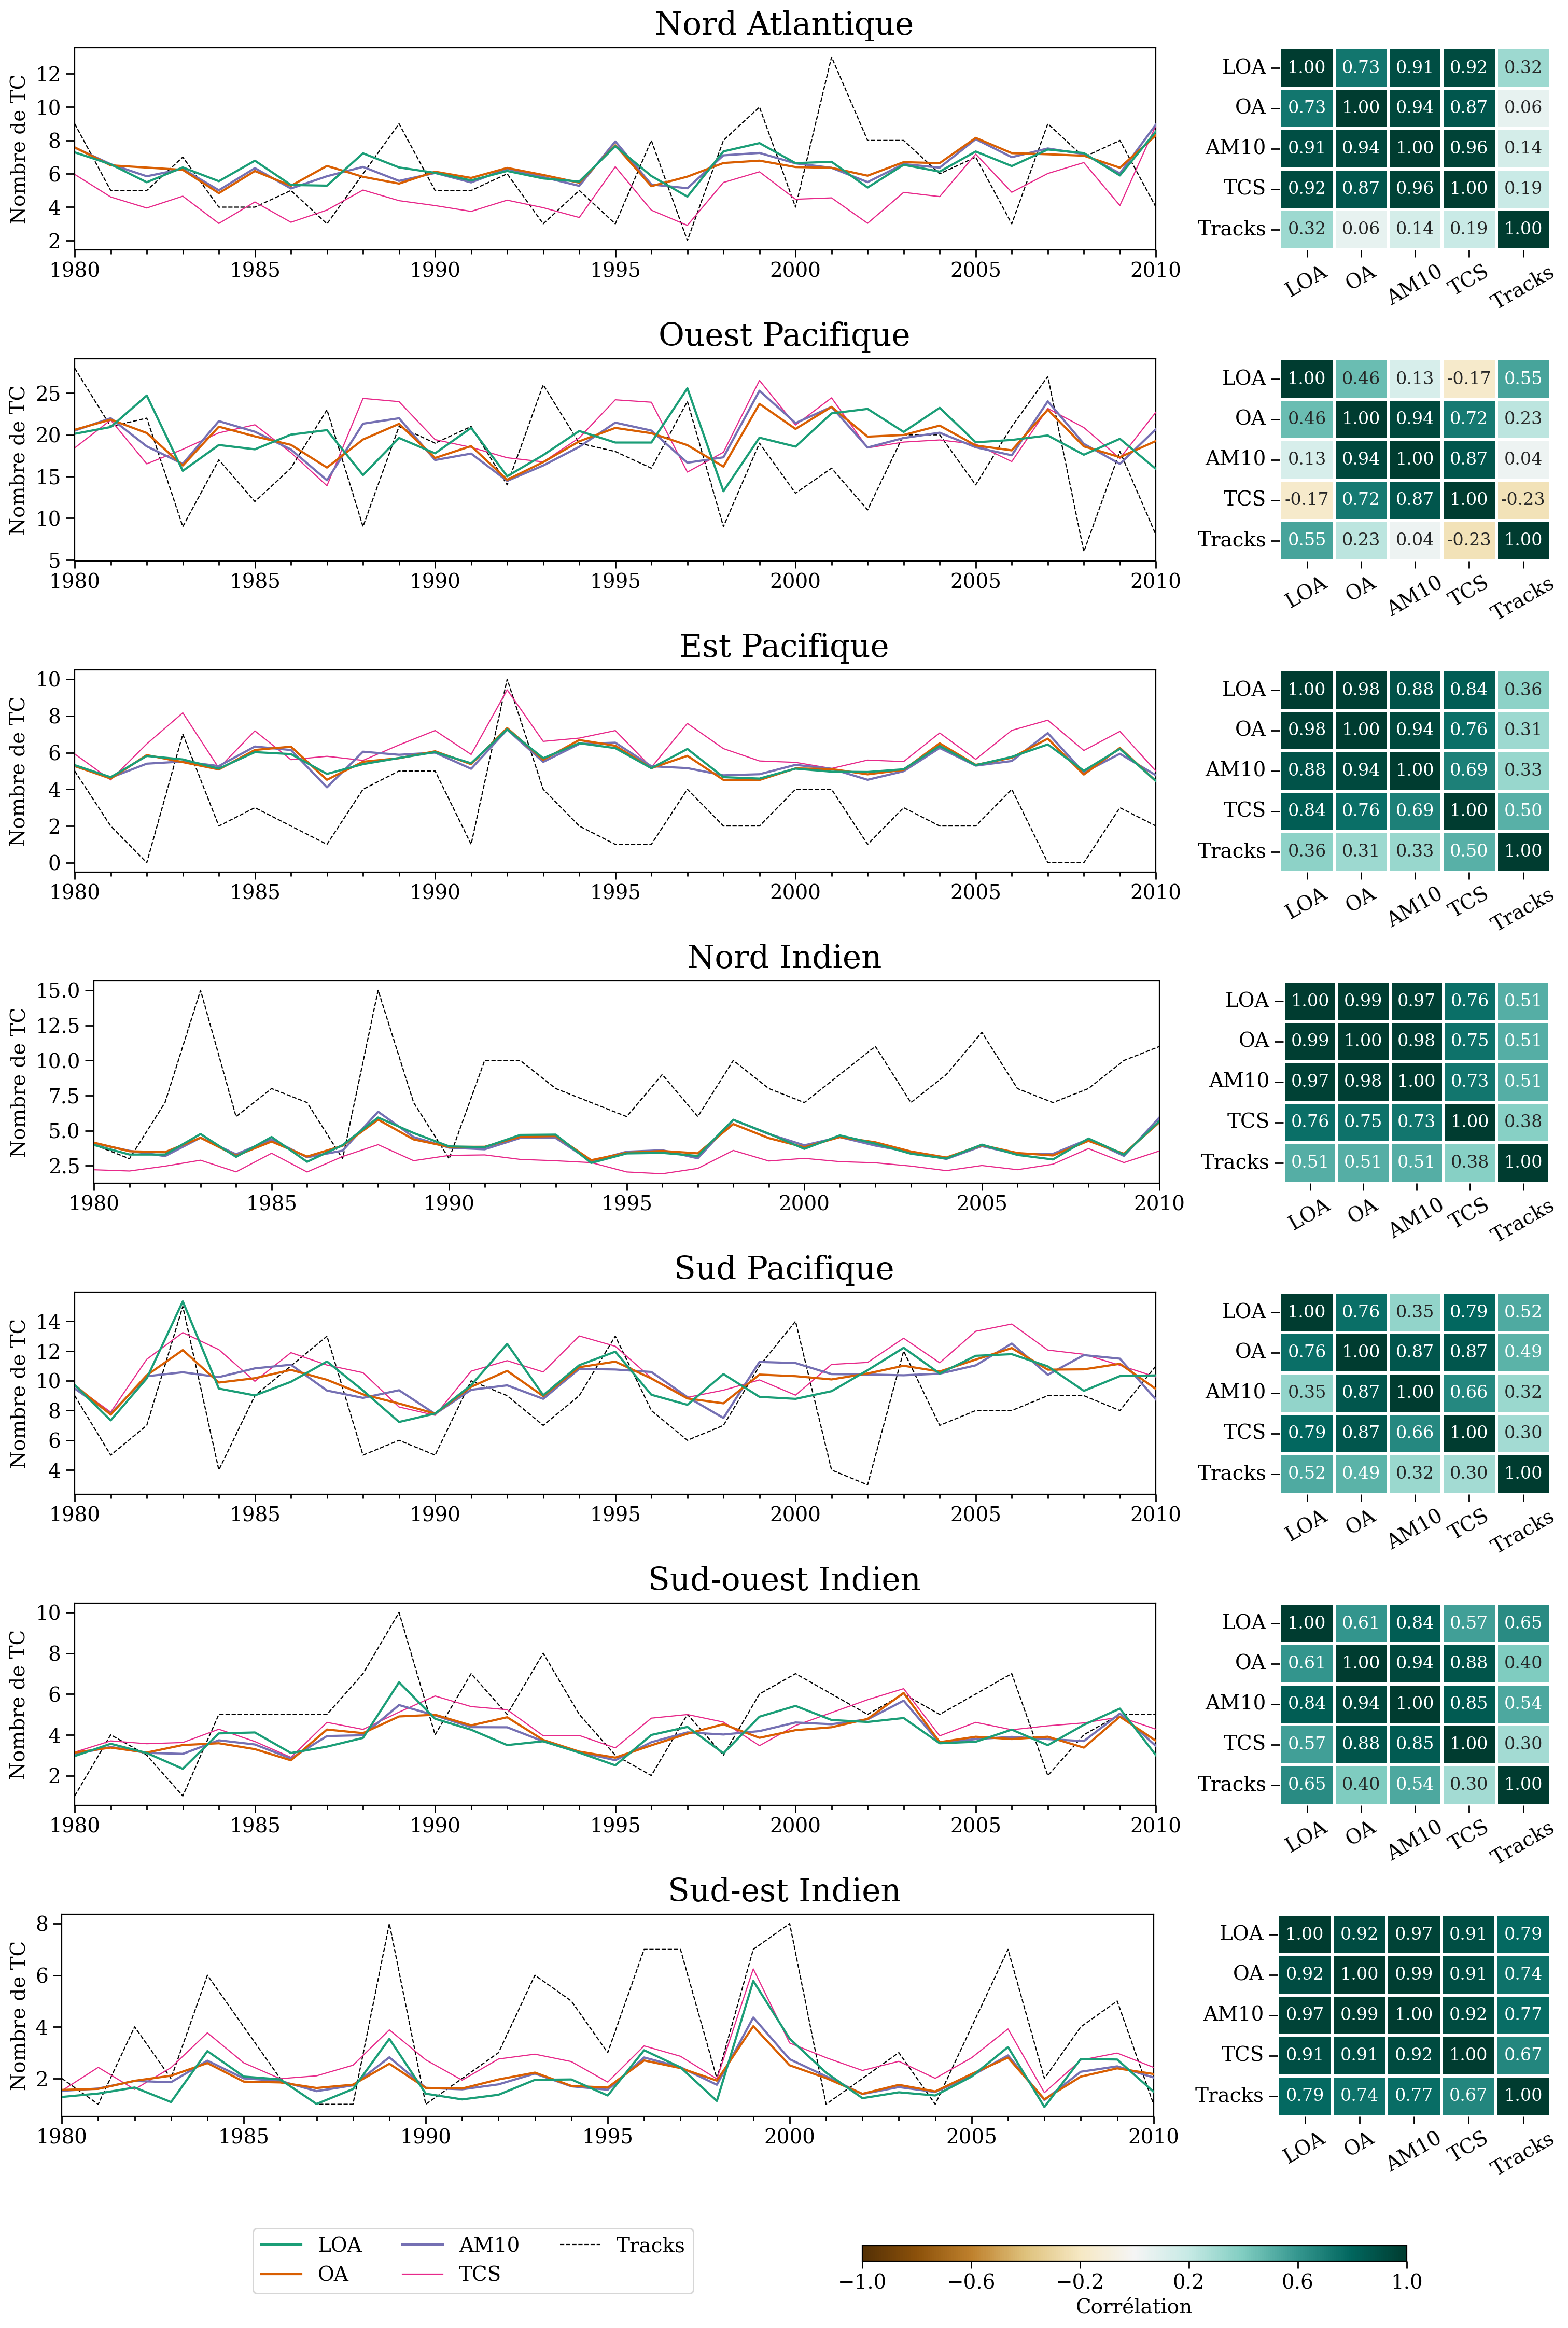
\includegraphics[height=0.94\textheight]{basin_variability_LOA_OA_AM10_TCS_Obs.png}
    \caption{Variabilité interannuelle des trois indices construits sur la simulation ARPEGE, du TCS et issue du schéma de détection (Tracks), ainsi que les
    matrices de corrélation associées.}
    \label{fig:variability_ONI}
\end{figure}

\begin{table}[htpb]
    \centering
    \caption{valeurs-p associées aux corrélations entre la variabilité interannuelle des indices et le tracking (dernière ligne, ou colonne, des matrices de
    corrélation de la \cref{fig:variability_ONI}). Les valeurs renseignées en gras indiquent les valeurs-p en dessous du seuil de \num{0.05}.}
    \label{tab:pvalues_ONI}
    \begin{tabular}{lrrrrrrr}
        \toprule\toprule
        \multicolumn{1}{c}{Indice} & \multicolumn{7}{c}{Bassin géographique}\\
        \midrule
                                   & NAtl & WPac & EPac & NInd & SPac & SIndW & SIndE \\
        \midrule
        LOA  & \num{0.084} & \textbf{\num{0.001}} & \textbf{\num{0.045}} & \textbf{\num{0.003}} & \textbf{\num{0.002}} & $\mathbf{< 10^{-3}}$ & $\mathbf{< 10^{-3}}$ \\
        OA   & \num{0.747} & \num{0.213} & \num{0.086} & \textbf{\num{0.003}} & \textbf{\num{0.005}} & \textbf{\num{0.026}} & $\mathbf{< 10^{-3}}$ \\
        AM10 & \num{0.438} & \num{0.839} & \num{0.069} & \textbf{\num{0.003}} & \num{0.077} & \textbf{\num{0.002}} & $\mathbf{< 10^{-3}}$ \\
        TCS  & \num{0.307} & \num{0.214} & \textbf{\num{0.004}} & \textbf{\num{0.036}} & \num{0.097} & \num{0.097} & $\mathbf{< 10^{-3}}$ \\
        \bottomrule
    \end{tabular}
\end{table}

La \cref{fig:variability_ONI} montre que l'ajout de l'indice ENSO comme prédicteur dans la régression parvient, avec un effet variable selon les bassins, à
modifier la variabilité interannuelle inférée par les indices de cyclogénèse d'une part, et à améliorer la corrélation entre cette variabilité et celle mesurée
par le schéma de détection de cyclones tropicaux dans la simulation ARPEGE d'autre part. Notons que le nombre annuel de TC simulé par l'indice LOA est significativement
corrélé à l'activité détectée par le traqueur dans tous les bassins géographiques à l'exception du Nord Atlantique. Dans ce dernier, le LOA présente néanmoins
une amélioration sensible de la corrélation associée à une valeur-p en limite de significativité par rapport aux autres indices.

L'impact le plus marquant se trouve dans le bassin Ouest Pacifique. La corrélation ---~quasi-nulle pour AM10, et négative pour TCS~--- passe de \num{0.23} pour
OA à \num{0.53} pour LOA. La corrélation entre le LOA et les tracks est hautement significative avec une valeur-p de \num{0.001}. Rappelons que le prédicteur
ONI présente également la significativité la plus élevée dans la régression de Poisson pour ce bassin (\cref{tab:coefs_LOA}) et aussi le coefficient
$b_{\mathrm{ONI}}$ le plus élevé. Les performances intermédiaires de l'indice OA proviennent alors sans doute de la sensibilité diminuée de l'indice à ce
prédicteur dans la régression globale. La valeur du coefficient $b_{\mathrm{ONI}}$ est en effet le coefficient présentant le plus grand changement entre
l'indice global OA et l'indice régional LOA, avec une sensibilité à la variable ONI \num{3.4} supérieure dans l'indice LOA par rapport à l'indice OA.

Les bassins SPac et SIndW voient également une amélioration sensible de leur variabilité interannuelle lorsque le prédicteur ONI est introduit dans la
régression régionale. Notons que dans ces deux bassins, la corrélation est significative pour OA et LOA, mais que la corrélation est diminuée pour OA par
rapport à AM10 dans le SIndW. L'indice LOA dépasse en revanche la corrélation de l'indice AM10. Dans le SPac, la corrélation temporelle de l'indice OA est
intermédiaire entre AM10 et LOA. Cela provient du fait que la variabilité ENSO est anti-corrélée dans le Sud Indien, et corrélée dans le Sud Pacifique, tandis
que le signe de $b_{\mathrm{ONI}}$ dans l'indice OA imprime un lien positif entre El Niño et l'activité cyclonique. Ainsi, bien que OA soit significativement
corrélé aux tracks dans le SIndW, la significativité est sensiblement plus marquée pour LOA dans ce bassin, avec une valeur-p inférieure à \num{1e-3}, et un
coefficient de corrélation parmi les plus élevés de tous les bassins de \num{0.65}, malgré un défaut d'amplitude.

Dans le SIndE et NInd, tous les indices sont significativement corrélés aux tracks. Dans le NInd, la corrélation est invariante entre AM10, OA et LOA, et les
séries temporelles indiscernables. Tous trois présentent néanmoins une amélioration par rapport au TCS. Notons que les valeurs du coefficient $b_{\mathrm{ONI}}$
entre OA et LOA sont proches l'une de l'autre, et particulièrement basses. Il n'est donc pas surprenant de ne voir aucun impact de l'ajout de la variable ONI
par rapport à AM10. Cette région fait partie de celles ---~avec le bassin EPac~--- pour lesquelles les cyclogénèses détectées par le traqueur dans ARPEGE
présentent un biais positif (négatif pour le bassin EPac) prononcé par rapport à IBTrACS (voir \cref{fig:density_arpege_ibtracs}). Ce biais est d'ailleurs
apparent sur la \cref{fig:variability_ONI} puisque tous les indices sous-estiment largement l'activité issue du traqueur dans la région. Dans le SIndE, on note
le même phénomène que dans le SIndW ; à savoir une amélioration entre AM10 et TCS, une dégradation entre OA et AM10 et de nouveau une amélioration pour LOA par
rapport aux trois autres. Cet effet s'explique de la même manière que pour le SIndW, mais il convient de noter que les différences dans les performances des
trois indices sont nettement moins prononcées que dans le bassin SIndW.

Le bassin EPac se démarque quelque peu des autres bassins puisque le TCS se place en première position, et dont la significativité est la plus franche avec une
valeur-p de \num{0.004}. Outre le TCS, seul l'indice LOA atteint également la significativité avec une valeur-p de \num{0.045}, mais un coefficient de
corrélation moindre par rapport à ce dernier. Comme mentionné précédemment, l'activité cyclonique détectée dans le modèle ARPEGE dans ce bassin présente un
important biais négatif. Il est alors possible que ce biais soit lié aux mauvaises performances des indices construits à partir des cyclogénèses détectées.

Enfin, notons que l'amplitude de la variabilité interannuelle simulée par les indices de cyclogénèse dans la plupart des bassins est sous-estimée. L'amplitude
dans le bassin WPac est la plus ressemblante à l'activité détectée, suivie du bassin SPac, notamment pour l'indice LOA. Une explication possible à cela pourrait
trouver son origine dans la nature même de la régression de Poisson. Rappelons en effet que les coefficients de la régression expriment des sensibilités de la
fréquence d'occurrence attendue des TC aux changements dans les prédicteurs. En particulier, ces sensibilités expriment une modification relative de la
fréquence modélisée par la régression. Ainsi, les deux régions les plus actives que sont les bassins WPac et SPac, dans lesquels les indices AM10, OA et LOA
produisent respectivement \num{19.4} TC par an et \num{10.12} TC par an\footnote{La fréquence d'occurrence moyenne simulée par le TCS n'est pas toujours alignée
sur celle des trois autres indices, selon les régions. Ce dernier est néanmoins également calibré pour produire \num{52.32} TC par an à l'échelle
globale.}\footnote{Rien n'impose que la fréquence d'occurrence moyenne de l'indice AM10 dans chacun des bassins soit égale à celle des indices OA et LOA. La
proximité entre les coefficients des deux indices ainsi que la faible sensibilité au prédicteur ONI dans l'indice OA laissent toutefois penser que les
fréquences moyennes régionales sont très proches, ce qui est également corroboré par la \cref{fig:variability_ONI}.} (\cref{tab:coefs_LOA}) présentent également
la plus grande amplitude. Inversement, les bassins où l'activité inférée par les indices est faible tendent à présenter une faible amplitude.

\subsection{Discussion}

Cette section s'est concentrée sur l'introduction d'un diagnostique du mode de variabilité El Niño dans la construction d'un indice de cyclogénèse par
régression de Poisson. Pour cela une simulation réalisée avec le modèle ARPEGE-Climat sur la période \num{1979}~--~\num{2010}, forcée par le jeu de données
HadISST1 est utilisée pour fournir les prédicteurs de grande échelle. Le schéma de détection du CNRM est utilisé pour comptabiliser les cyclogénèses dans la
simulation, lesquelles étant préalablement filtrées par le diagnostique du jet subtropical présenté dans le \cref{chap:chapitre_2}. La répartition spatiale de
l'activité cyclonique détectée dans la simulation ARPEGE est jugée suffisamment réaliste pour utiliser ces données comme prédictant dans une régression de
Poisson, malgré un biais négatif important dans le bassin Est Pacifique, et un biais au contraire positif dans le bassin Nord Indien (voir
\cref{sec:tracking_arpege}). L'utilisation du diagnostique ENSO dans la construction d'indices de cyclogénèse consiste à apporter artificiellement, et de la
manière la plus explicite possible, l'information concernant la phase du mode de variabilité océanique dans la régression, de façon à ce que chaque point de
grille ait accès à cette information à chaque pas de temps.

Trois indices sont construits sur les champs mensuels de la simulation interpolés sur une grille régulière de \ang{1} de résolution horizontale : Un indice
global basé sur les prédicteurs du TCS (AM10), un indice global similaire auquel est ajouté la variable ONI (OA) et un indice régional ---~c'est à dire dont les
coefficients sont fonction du bassin océanique~--- possédant lui aussi la variable ONI comme prédicteur (LOA). La régionalisation de l'indice avec l'ONI est en
effet jusitifée par le fait que l'effet du phénomène El Niño sur la modulation de l'activité cyclonique est positif dans certaines régions, et négatif dans
d'autres (voir \cref{sec:lien_enso_tracking}). Les résultats montrent que l'ajout de la variable ONI comme prédicteur dans la construction de l'indice parvient
efficacement à améliorer la représentation de la variabilité interannuelle inférée par l'indice de cyclogénèse régional, avec l'impact le plus frappant
concernant le bassin Ouest Pacifique. Seules les deux régions dans lesquelles l'activité cyclonique simulée par ARPEGE présente un biais important ne montrent
pas d'amélioration notable suite à l'introduction de ce nouveau prédicteur. Cette amélioration de la variabilité interannuelle se fait cependant au détriment du
sens physique que porte sinon l'indice de cyclogénèse, la philosophie originelle consistant en effet à n'utiliser que des variables intervenant (supposément)
directement dans le processus physique de cyclogénèse.

L'amélioration de la variabilité interannuelle lorsque la phase du mode de variabilité El Niño est explicitement renseignée interroge également sur la manière
dont un indice de cyclogénèse perçoit les télé-connexions. En effet, l'activité cyclonique simulée par le modèle atmosphérique ressent l'effet de l'ENSO, comme
en atteste la \cref{sec:lien_enso_tracking} (et notamment les \cref{fig:corr_ONI_pt,fig:corr_ONI_bassin}). \textcite{camargo_use_2007} montrent par ailleurs que
le GPI de \textcite{emanuel_tropical_2004} reproduit fidèlement les anomalies spatiales de l'activité cyclonique liées à l'ENSO, et mettent en évidence
l'importance du rôle joué par chacun des prédicteurs, notamment de l'humidité relative en moyenne troposphère et le cisaillement vertical du vent. Ces
variables, ainsi que la SST (absente du GPI), faisant partie intégrante des indices utilisés ici, une bonne réponse dans la variabilité interannuelle de ces
derniers à la phase de l'ENSO pouvait être attendue. De surcroît, la variabilité interannuelle des indices utilisés ici n'incluant pas la variable ONI, à savoir
l'AM10 et le TCS, réagissent tout de même à la phase de l'ENSO, mais dans une mesure amoindrie et de manière moins consistante. On peut en effet le voir pendant
l'épisode de 1983 dans le bassin SPac, mais aussi en 1992 et 1997 dans le bassin EPac et ainsi qu'en 1999 dans le bassin SIndE, pour ne citer que quelques
exemples. La capacité des indices de cyclogénèse à réagir à ce mode de variabilité est en outre documentée depuis les travaux de
\textcite{watterson_seasonal_1995} (c.f \cref{sec:intro_indices} du \cref{chap:chapitre_1}).

Sachant cela, l'introduction de la variable ONI aurait pu être tout à fait redondante et n'apporter aucune plus-value dans la régression. C'est d'ailleurs une
interprétation possible aux significativités pour le moins hésitantes associées à ce prédicteur dans le \cref{tab:coefs_LOA}. En effet, le champ spatial
artificiel de l'ONI, construit en répliquant la valeur (scalaire) du diagnostique en tout point de l'espace, ne contient par définition aucune variabilité
spatiale. Or, les résultats obtenus dans le \cref{chap:chapitre_3} montrent que la régression de Poisson vise avant toute autre chose à fournir la meilleure
vraisemblance spatiale entre les prédicteurs et le prédictant. Malgré cela, l'utilisation de l'ONI comme prédicteur et d'un coefficient $b_{\mathrm{ONI}}$
associé, quand bien même ce dernier n'est pas statistiquement significatif, améliore sensiblement la corrélation entre la variabilité interannuelle de l'indice
avec la variabilité détectée dans la plupart des bassins. Chercher à améliorer la représentation de la variabilité interannuelle inférée par un indice de
cyclogénèse par l'ajout de nouveaux prédicteurs apparaît donc possible, mais la méthodologie de construction d'un indice par régression de Poisson ne semble pas
être le mode opératoire le mieux adapté à cette tâche.

% Rappelons également que la significativité associée à la variable ONI dans l'indice régional ne reflète pas nécessairement celle entre la série temporelle de
% l'ONI et la variabilité temporelle de l'activité détectée dans la simulation (c.f \cref{fig:corr_ONI_bassin}), avec notamment un lien clair entre ENSO et les
% cyclogénèses détectées dans les bassins SIndW et SIndE, mais moins évident dans le SPac, tandis que l'ajout du prédicteur dans ces régions pour la construction
% de l'indice LOA renvoie le message inverse. Une explication à ce qui peut alors

\section{Introduction du déficit de saturation d'humidité}\label{sec:tendances_VPD}

Le déficit de saturation d'humidité atmosphérique, comme déjà évoqué dans le \cref{chap:chapitre_1} (\cref{sec:projections_futures}), constitue une variable
d'intérêt pour l'étude de l'activité cyclonique tropicale dans le contexte de réchauffement climatique. Dans une atmosphère plus chaude, celui-ci augmente du
fait de la dépendance de la pression de vapeur saturante à la température, tandis que l'humidité relative est projetée comme approximativement constante. Le
déficit de saturation d'humidité, que l'on appelera par la suite VPD (\textit{Vapour-Pressure Deficit}), et noté $s$, est défini ici comme la différence $s =
e_s - e$, où $e_s$ est la pression de vapeur saturante et $e$ la pression partielle de la vapeur d'eau : $e / e_s$. Le VPD se distingue donc de l'humidité
relative définie par le ratio entre la pression partielle de la vapeur d'eau et la pression de vapeur saturante. \textcite{emanuel_hurricanes_2008} montrent via
une expérience de descente d'échelle statistique que des simulations climatiques dans lesquelles le déficit de saturation est maintenu constant présentent une
augmentation du nombre de TC, alors qu'elles indiquent sinon une baisse lorsque ce paramètre n'est pas influencé. Ces résultats ont conduit à la formulation
modifiée du GPI proposée par \textcite{emanuel_tropical_2010} ---~mentionnée dans la \cref{sec:relations_empiriques} du \cref{chap:chapitre_3}~--- dans laquelle
l'humidité relative est remplacée par une mesure adimensionnelle du déficit de saturation d'entropie humide, similaire au VPD. Cet indice appliqué aux
simulations CMIP5 présente cependant toujours un signal divergeant (c'est à dire une augmentation de l'activité) en climat plus chaud.
\textcite{camargo_testing_2014} montrent à l'inverse que certaines combinaisons de prédicteurs dans un indice de cyclogénèse construit par régression de Poisson
peuvent aboutir à une fréquence d'occurrence à la baisse en climat futur, notamment lorsque le VPD est introduit.

On s'intéresse dans cette nouvelle et dernière section à l'apport du VPD en lieu et place de l'humidité relative à \hPa{600} dans un indice de cyclogénèse
construit par une régression de Poisson. En particulier, puisqu'il a été mis en évidence que la variabilité interannuelle d'un tel indice était difficile à
améliorer, nous nous intéressons plutôt à la recherche et à l'analyse de tendances dans la variabilité du nombre de TC d'une année sur l'autre.

\subsection{Régression de Poisson avec le VPD}

Conformément à \textcite{camargo_testing_2014}, le VPD est intégré verticalement en chaque point de grille. L'intégration verticale bénéficie en effet de
l'avantage, par rapport à une moyenne, de ne pas être influencé par les valeurs très faibles dans les dernières couches de l'atmosphère. Le déficit de
saturation d'humidité s'exprime traditionnellement en \SI{}{\kilo\pascal}, et l'intégrale sur plus d'une vingtaine de niveaux verticaux d'espacement variable
amène à de larges valeurs numériques. Pour cette raison, le VPD intégré sur la colonne est exprimé ici en $10^6$~\SI{}{\pascal\squared}. Cela se traduit par une
plage de valeurs comprise entre \SI{1e6}{\pascal\squared} et \SI{62e6}{\pascal\squared}, soit un ordre de grandeur comparable aux autres prédicteurs, et en
particulier à l'humidité relative ---~que le VPD remplace~--- et donc \textit{in fine} à une valeur du coefficient $b_s$ qu'il est possible de comparer à $b_H$.
En effet, puisque les coefficients expriment des sensibilités pour des changements unitaires, l'application d'un facteur d'échelle au prédicteur se répércute de
la même manière sur son coefficent dans la régression. En outre, et bien que \textcite{camargo_testing_2014} ne précisent pas l'unité utilisée pour le déficit
de saturation intégré sur la colonne, notre valeur de $b_s$ est du même ordre de grandeur que celle proposée pas ces derniers.

La régression est faite selon l'exact même mode opératoire que pour l'indice AM10 construit dans la section précédente, et l'indice M10 établit sur ERA5 avant
lui (voir \cref{sec:apport_res_temporel_spatial}). La relation ainsi établie est donnée ci-dessous :
%
\begin{align*}
\tag{AVPD}
    \mu &= \exp \big( b_0 + b_\eta \eta + b_{V_{\mathrm{shear}}} V_{\mathrm{shear}} + b_{s} \, s + b_T T + \log \cos \phi \big)\\
        &= \exp \big( \num{-13.5399} + \num{2.3765} \, \eta - \num{0.0179} \, V_{\mathrm{shear}} \underbrace{- \num{0.1238} \, s}_{\mathrm{VPD}} + \num{0.6204} \, T + \log \cos \phi \big)
\end{align*}
%
Le coefficient $b_s$ est donné à \mypm{-0.1238}{0.007}, avec des pourcentiles \prct{2.5} et \prct{97.5} de respectivement \num{-0.138} et \num{-0.110}. Le
prédicteur est donc hautement significatif dans la régression. À titre de référence, le coefficient trouvé dans \textcite{camargo_testing_2014}, entre la
réanalyse NCEP et IBTrACS, est de $+$\num{0.13}. La différence du signe s'explique par le fait qu'ici, et contrairement à \textcite{camargo_testing_2014}, le
VPD est défini positif, si bien qu'une grande valeur de $s$ est associée à une colonne atmosphérique particulièrement sèche, et donc défavorable à la
cyclogénèse. Notons que la régression faite sur ERA5 et IBTrACS (protocole M10) avec l'intégrale verticale du VPD en remplacement de l'humidité relative conduit
à une valeur similaire avec $b_s^{\mathrm{ERA5}} \sim \num{-0.17}$. Avec les moyennes climatologiques (protocole C10), on a $b_s^{\mathrm{ERA5}} \sim
\num{-0.14}$, ce qui se rapproche encore d'avantage du coefficient de \textcite{camargo_testing_2014}, lesquels utilisent également des moyennes
climatologiques. Ici, les coefficients $b_\eta$ et $b_{V_{\mathrm{shear}}}$ demeurent quasiment inchangés par rapport à AM10. La seule différence notable se
trouve dans la sensibilité à la SST relative, qui passe d'environ \num{0.42} à \num{0.62} ici. Une augmentation du même ordre de grandeur est notée sur ERA5
(M10 comme C10), avec par exemple un passage de $b_T^{\mathrm{ERA5}}$ de \num{0.41} à \num{0.62} pour M10. \textcite{camargo_testing_2014} présentent le même
constat avec un coefficient de SST relative passant de \num{0.35} à \num{0.57} lorsque le VPD est introduit. L'effet du VPD sur les coefficients de la
régression entre la fréquence d'occurrence des TC et l'environnement de grande échelle apparaît donc robuste entre NCEP, ERA5 et les observations IBTrACS d'un
côté, et notre simulation ARPEGE forcée par HadISST1 et les cyclogénèses issues du schéma de détection de cyclones tropicaux de l'autre.

Précisons que l'introduction du VPD dans la régression de Poisson n'a que peu d'impact sur la variabilité interannuelle. En outre, la corrélation de la
variabilité interannuelle inférée par l'indice AVPD est généralement inchangée par rapport à AM10, mais peut également être dégradée, comme en atteste la
\cref{fig:corr_AVPD_AM10_M10}. Contrairement à l'introduction de l'indice ONI dans la \cref{sec:indice_ONI}, aucun bassin ne voit sa corrélation entre la
variabilité interannuelle de l'indice et celle du traqueur devenir significative grâce à l'introduction du VPD.

\begin{figure}[htb]
    \centering
    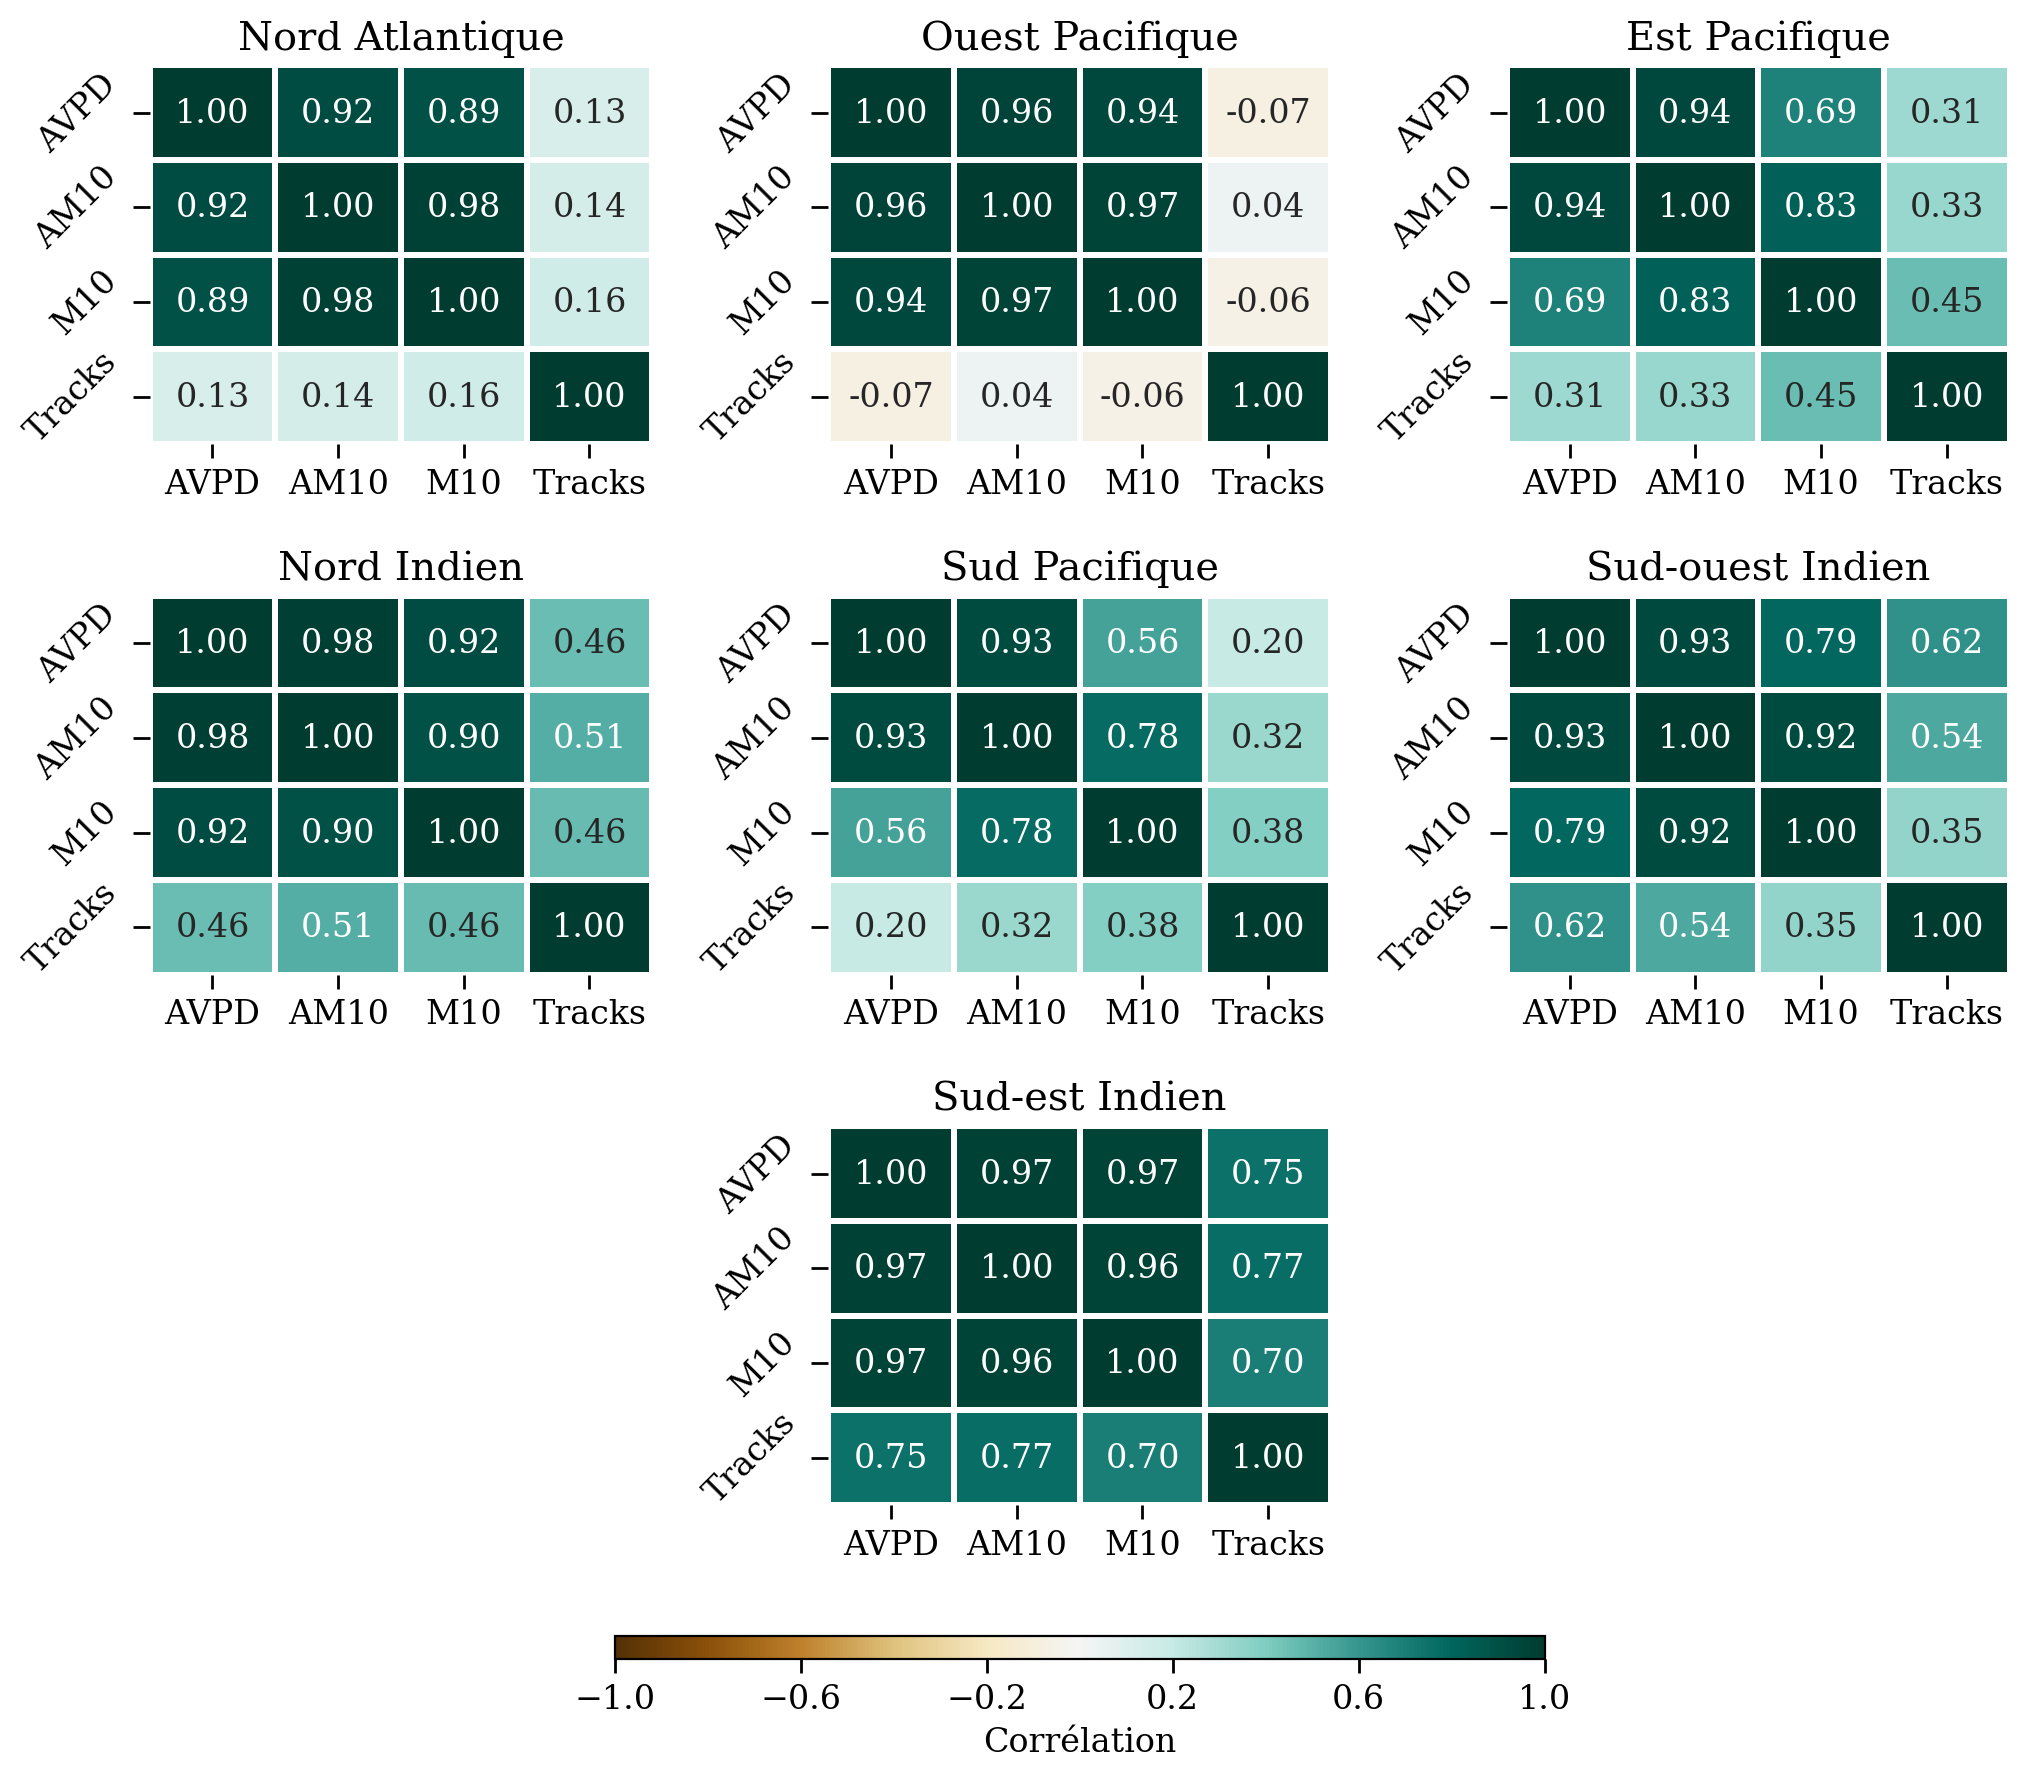
\includegraphics[width=\textwidth]{corr_AVPD_AM10_M10_tracks.png}
    \caption{Corrélations croisées entre la variabilité interannuelle de : AVPD ; AM10 ; M10 du \cref{chap:chapitre_3} appliqué à la simulation ARPEGE ; le
    schéma de détection, entre 1980 et 2010.}
    \label{fig:corr_AVPD_AM10_M10}
\end{figure}

La \cref{fig:diff_VPD_AM10} présente la différence entre les moyennes temporelles de l'indice AVPD et l'indice AM10. L'effet du VPD dans la répartition spatiale
de l'activité simulée par l'indice est variable selon les bassins (voir aussi le \cref{tab:tendances_PRE625REFT359x} pour la façon dont la fréquence annuelle
est affectée par ce nouveau prédicteur dans chacun des bassins). Le VPD amène notamment à deux changements intéressants, présentés dans les grossissements sur
la \cref{fig:diff_VPD_AM10}. Ces deux régions correspondent à des domaines où ni IBTrACS, ni les cyclogénèses détectées dans ARPEGE ne recensent d'activité
(voir \cref{fig:acgi_ibt,fig:track_density_PRE625REFT359x}). Par conséquent, toute activité simulée par un indice de cyclogénèse construit sur ces données
constitue nécessairement un biais de l'indice\footnote{Les indices de cyclogénèse présentés dans ce manuscrit ne sont par définition jamais strictement nuls, ce
qui est d'autant plus vrai pour les régressions de Poisson définis comme une fonction exponentielle. Dans les régions évoquées, il ne fait toutefois aucun
doute que le niveau d'activité des indices dépasse celui d'un simple bruit de fond.}. Or, un tel biais est présent dans le GPI et le TCS (de même que tous les
indices dérivés du TCS définis dans ce manuscrit jusqu'à maintenant, et notamment AM10), mais pas le CYGP, lequel ---~rappelons le~--- ne dépend pas de
l'humidité relative. Ce biais est brièvement mentionné dans le \cref{chap:chapitre_3} (\cref{sec:proprietes_indices}).

\begin{figure}[tb]
    \centering
    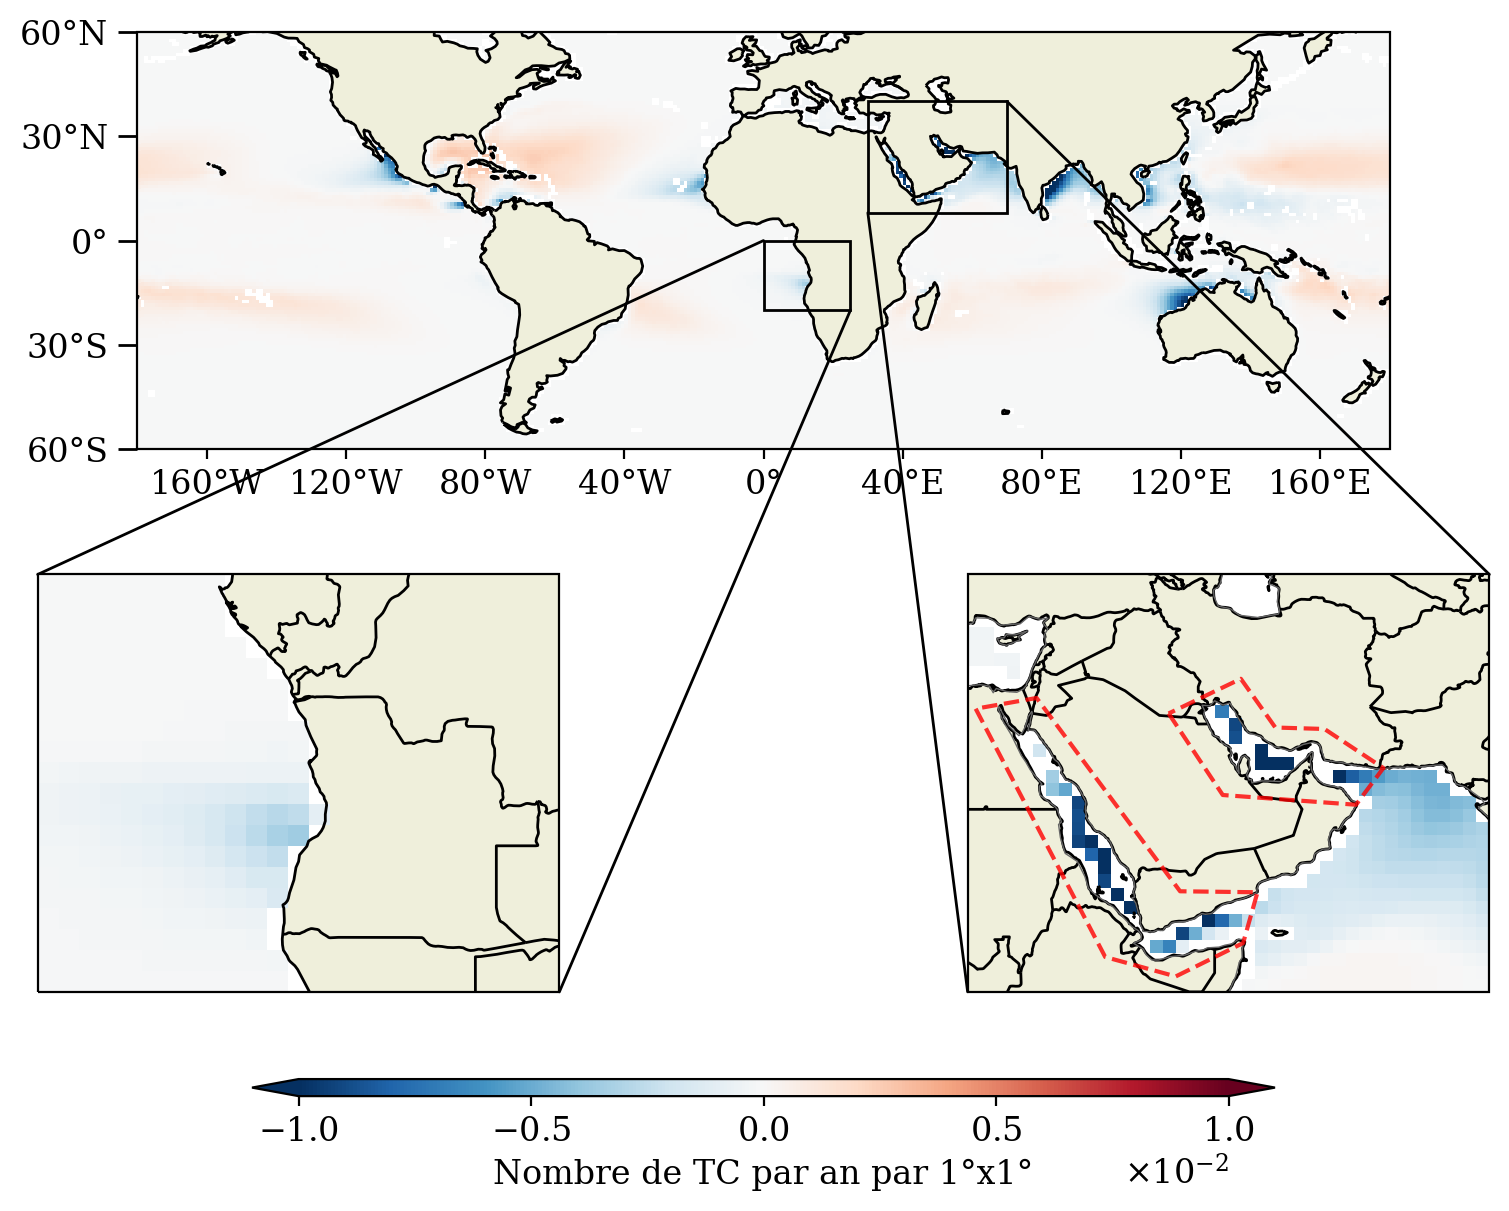
\includegraphics[width=\textwidth]{carte_diff_VPD_AM10.png}
    \caption{Carte des différences annuelles moyennes entre l'indice AVPD et AM10. Les deux grossissements montrent la côte au large de l'Angola (entre \ang{0}E
    et \ang{25}E, et \ang{20}S et l'équateur) d'une part et la région du Golfe Persique et de la Mer Rouge (entre \ang{30}E et \ang{70}E, et \ang{8.5}N et
    \ang{40}N) d'autre part.}
    \label{fig:diff_VPD_AM10}
\end{figure}

Le premier changement, et le plus conséquent des deux, consiste en la réduction du biais positif dans le Golfe Persique ainsi qu'en Mer Rouge, deux sous-régions
du bassin NInd. En Mer Rouge (incluant le Golfe d'Aden, entre le Yémen et la Somalie, délimitée en pointillés sur la \cref{fig:diff_VPD_AM10}), la fréquence
annuelle moyenne entre \num{1980} et \num{2010} inférée par l'indice AM10 est de \num{0.2} TC par an, tandis qu'elle est réduite à \num{0.02} TC par an pour
l'indice incluant le VPD. Réciproquement, dans le Golfe Persique (en incluant également le Golfe d'Oman à l'embouchure, voir délimitations en pointillés), la
fréquence est réduite de \num{0.1} TC par an à \num{0.005} TC par an pour l'indice incluant le VPD par rapport à AM10. . Il en résulte que la production de TC
dans ces régions est purement une conséquence de l'utilisation de l'humidité relative dans la formulation des indices. Le deuxième domaine dont la
représentation de l'activité est amélioré par l'introduction du VPD est au large des côtes de l'Angola. L'indice incluant le VPD voit sa fréquence réduite de
\num{0.13} TC par an (AM10, le TCS y simule quant à lui \num{0.17} TC par an) à \num{0.03} TC par an. Cette région ne présente pas d'activité cyclonique dans
les observations, ni dans les données du traqueur, mais tous les indices dépendant de l'humidité relative y présentent un bias positif, si bien que toute
réduction de l'activité représente une amélioration.

\subsection{Détection de tendances dans ARPEGE et ERA5}

Le \cref{tab:tendances_PRE625REFT359x} présente l'analyse des tendances dans le nombre annuel de TC dans la simulation ARPEGE forcée par HadISST1 ainsi que dans
la réanalyse ERA5, tels que vus par plusieurs indices et par le schéma de détection (ou dans le cas d'ERA5, par IBTrACS). L'indice dans lequel le VPD remplace
l'humidité relative y est appelé AVPD pour celui dont la régression est faite entre ARPEGE et le schéma de détection, et EVPD pour celui dont la régression est
faite sur ERA5 avec IBTrACS. Sont également inclus dans ce tableau : l'indice AM10 (non appliqué à ERA5) ; l'indice M10 du \cref{chap:chapitre_3}, évalué sur
ERA5 comme sur la simulation ARPEGE historique ; le TCS et enfin les données issues du schéma de détection / IBTrACS. La comparaison avec M10 en plus du TCS se
justifie par le fait que l'indice M10 peut être vu comme une version actualisée du TCS. En revanche, appliquer la relation AM10 à ERA5 n'aurait pas beaucoup de
sens. Pour les tendances évaluées sur ERA5, la période \num{1981}~--~\num{2011} est prise pour disposer de \num{31} saisons cycloniques dans les deux jeux de
données. C'est pour cette raison que la fréquence annuelle globale dans ERA5 est différente de la valeur de calibration, celle-ci étant établie sur la base de
la saison 2019 comme borne supérieure.

\begin{table}[htpb]
    \centering
    \caption{ Tendances (TC par décennie) et valeur-p associées dans la simulation ARPEGE forcée par HadISST1 entre 1980 et 2010, ainsi que dans ERA5 entre 1981
    et 2011. Les lignes en gras désignent une tendance significative à \prct{95}. La colonne Fréquence indique la fréquence annuelle moyenne en TC par an.}
    \label{tab:tendances_PRE625REFT359x}
    \begin{adjustbox}{height=0.45\textheight}
        \begin{tabular}{llrrr|rrr}
        \toprule
         &  & \multicolumn{3}{r}{\textbf{ARPEGE}} & \multicolumn{3}{r}{\textbf{ERA5}} \\
         &  & Pente & valeur-p & Fréquence & Pente & valeur-p & Fréquence \\
        \cline{1-8}
        \multirow[t]{7}{*}{\textbf{Nord Atlantique}} & AVPD & 0,214 & 0,276 & 7,1 & --- & --- & --- \\
         & EVPD & --- & --- & --- & 0,440 & 0,143 & 8,0 \\
         & AM10 & \textbf{0,446} & \textbf{0,018} & \textbf{6,4} & --- & --- & --- \\
         & M10 & \textbf{0,602} & \textbf{0,011} & \textbf{4,7} & \textbf{0,871} & \textbf{0,007} & \textbf{8,6} \\
         & TCS & \textbf{0,645} & \textbf{0,014} & \textbf{4,7} & \textbf{1,131} & \textbf{0,003} & \textbf{8,9} \\
         & Tracks & 0,585 & 0,252 & 6,1 & --- & --- & --- \\
         & IBTrACS & --- & --- & --- & \textbf{3,198} & \textbf{0,001} & \textbf{12,4} \\
        \cline{1-8}
        \multirow[t]{7}{*}{\textbf{Ouest Pacifique}} & AVPD & -0,121 & 0,845 & 19,3 & --- & --- & --- \\
         & EVPD & --- & --- & --- & \textbf{2,245} & \textbf{0,010} & \textbf{29,6} \\
         & AM10 & 0,268 & 0,622 & 19,4 & --- & --- & --- \\
         & M10 & 0,407 & 0,527 & 21,0 & \textbf{2,909} & \textbf{0,000} & \textbf{28,8} \\
         & TCS & 0,467 & 0,458 & 19,9 & \textbf{2,571} & \textbf{0,002} & \textbf{30,0} \\
         & Tracks & -1,347 & 0,251 & 17,3 & --- & --- & --- \\
         & IBTrACS & --- & --- & --- & \textbf{-1,718} & \textbf{0,034} & \textbf{25,7} \\
        \cline{1-8}
        \multirow[t]{7}{*}{\textbf{Est Pacifique}} & AVPD & -0,191 & 0,297 & 5,5 & --- & --- & --- \\
         & EVPD & --- & --- & --- & \textbf{-1,556} & \textbf{0,040} & \textbf{17,5} \\
         & AM10 & -0,023 & 0,882 & 5,5 & --- & --- & --- \\
         & M10 & 0,079 & 0,712 & 6,3 & -0,819 & 0,265 & 17,1 \\
         & TCS & 0,018 & 0,934 & 6,3 & -1,123 & 0,191 & 16,0 \\
         & Tracks & -0,565 & 0,195 & 2,8 & --- & --- & --- \\
         & IBTrACS & --- & --- & --- & \textbf{-2,565} & \textbf{0,009} & \textbf{16,9} \\
        \cline{1-8}
        \multirow[t]{7}{*}{\textbf{Nord Indien}} & AVPD & -0,069 & 0,646 & 2,7 & --- & --- & --- \\
         & EVPD & --- & --- & --- & 0,034 & 0,703 & 3,0 \\
         & AM10 & 0,031 & 0,862 & 4,0 & --- & --- & --- \\
         & M10 & 0,048 & 0,753 & 2,9 & \textbf{0,324} & \textbf{0,015} & \textbf{4,0} \\
         & TCS & 0,071 & 0,529 & 2,8 & 0,133 & 0,218 & 3,6 \\
         & Tracks & 0,911 & 0,126 & 8,1 & --- & --- & --- \\
         & IBTrACS & --- & --- & --- & --- & --- & --- \\
        \cline{1-8}
        \multirow[t]{7}{*}{\textbf{Sud Pacifique}} & AVPD & 0,315 & 0,293 & 10,9 & --- & --- & --- \\
         & EVPD & --- & --- & --- & -0,052 & 0,922 & 14,0 \\
         & AM10 & \textbf{0,494} & \textbf{0,039} & \textbf{10,1} & --- & --- & --- \\
         & M10 & 0,579 & 0,063 & 10,5 & 0,250 & 0,588 & 12,7 \\
         & TCS & 0,478 & 0,138 & 10,9 & -0,217 & 0,708 & 12,7 \\
         & Tracks & 0,121 & 0,847 & 8,5 & --- & --- & --- \\
         & IBTrACS & --- & --- & --- & -0,964 & 0,220 & 10,5 \\
        \cline{1-8}
        \multirow[t]{7}{*}{\textbf{Sud-ouest Indien}} & AVPD & 0,138 & 0,359 & 4,3 & --- & --- & --- \\
         & EVPD & --- & --- & --- & -0,197 & 0,506 & 8,2 \\
         & AM10 & 0,274 & 0,061 & 3,9 & --- & --- & --- \\
         & M10 & \textbf{0,382} & \textbf{0,049} & \textbf{4,2} & -0,024 & 0,930 & 6,9 \\
         & TCS & \textbf{0,341} & \textbf{0,034} & \textbf{4,4} & -0,106 & 0,687 & 6,9 \\
         & Tracks & 0,391 & 0,336 & 4,9 & --- & --- & --- \\
         & IBTrACS & --- & --- & --- & 0,165 & 0,704 & 8,7 \\
        \cline{1-8}
        \multirow[t]{7}{*}{\textbf{Sud-est Indien}} & AVPD & 0,061 & 0,613 & 1,5 & --- & --- & --- \\
         & EVPD & --- & --- & --- & 0,057 & 0,808 & 3,7 \\
         & AM10 & 0,114 & 0,380 & 2,1 & --- & --- & --- \\
         & M10 & 0,175 & 0,351 & 2,2 & 0,114 & 0,679 & 4,7 \\
         & TCS & 0,175 & 0,351 & 2,7 & -0,062 & 0,795 & 4,6 \\
         & Tracks & 0,323 & 0,506 & 3,6 & --- & --- & --- \\
         & IBTrACS & --- & --- & --- & -0,649 & 0,288 & 7,6 \\
        \cline{1-8}
        \multirow[t]{7}{*}{\textbf{Global}} & AVPD & 0,332 & 0,743 & 52,3 & --- & --- & --- \\
         & EVPD & --- & --- & --- & 0,935 & 0,553 & 84,6 \\
         & AM10 & \textbf{1,633} & \textbf{0,045} & \textbf{52,3} & --- & --- & --- \\
         & M10 & \textbf{2,297} & \textbf{0,009} & \textbf{52,3} & \textbf{3,649} & \textbf{0,001} & \textbf{83,7} \\
         & TCS & \textbf{2,232} & \textbf{0,007} & \textbf{52,3} & \textbf{2,349} & \textbf{0,041} & \textbf{83,7} \\
         & Tracks & 0,129 & 0,932 & 52,3 & --- & --- & --- \\
         & IBTrACS & --- & --- & --- & -0,528 & 0,759 & 83,6 \\
        \bottomrule
        \end{tabular}
\end{adjustbox}
\end{table}

Dans le bassin NAtl, tous les indices basés sur l'humidité relative détectent une tendance à la hausse statistiquement significative. Dans ARPEGE, celles-ci
sont faibles, de l'ordre de \num{0.5} TC par décennie, tandis que le schéma de détection ne détecte pas de telle tendance, de même que l'indice AVPD. Dans ERA5,
les tendances sont plus marquées, mais les indices produisent également plus de TC dans ce bassin par rapport au modèle, du fait de leur calibration différente.
Rapportées à la fréquence annuelle moyenne, les tendances relatives sont en fait semblables entre ARPEGE et ERA5. Toutefois, IBTrACS présente une tendance à la
hausse plus importante, déjà mentionnée dans le \cref{chap:chapitre_1} (\cref{sec:observations}) et valant ici environ \num{3.2} TC par décennie. Cela tend
alors à donner raison au TCS et dérivés, tandis que les indices utilisant le déficit de saturation seraient mis en défaut dans ce bassin. Précisons néanmoins
qu'une tendance dans la fréquence annuelle de TC n'est pas détectée dans ARPEGE par le schéma de détection, si bien que l'absence de tendance dans l'indice AVPD
est au moins cohérente avec les tracks.

Les trois indices calculés sur ERA5 indiquent une tendance significative d'ampleur comparable dans le bassin WPac, entre \num{2.2} TC par décennie pour EVPD et
\num{2.9} TC par décennie pour M10. Dans IBTrACS, une tendance significative mais de signe opposée est identifiée à raison de \num{-1.7} TC par décennie. Il est
clair que la tendance positive dans ERA5 provient de la rupture liée à l'humidité dans le bassin WPac, largement documentée dans le \cref{chap:chapitre_3}.
L'indice EVPD est également concerné, car le déficit de saturation d'humidité intégré sur la colonne présente dans ERA5 une tendance opposée à celle de
l'humidité relative (donc à la baisse), si bien que la rupture dans la variabilité interannuelle de l'indice est toujours visible dans la réanalyse dans ce
bassin avec l'indice EVPD. Aucune tendance significative n'est identifiée dans ARPEGE, que ce soit dans les indices ou dans les tracks. Il est toutefois
possible que le traqueur indiquerait une tendance à la baisse significative dans une simulation plus longue, car celui-ci présente une pente de \num{-1.35} TC
par décennie (soit une tendance relative plus forte que dans IBTrACS) avec une valeur-p plus basse que celle des indices.

Dans le bassin EPac, l'indice EVPD présente une tendance du même signe qu'IBTrACS mais d'amplitude réduite, avec respectivement \num{-1.6} TC par décennie pour
EVPD et \num{-2.6} TC par décennie dans IBTracs. Aucun des indices basés sur l'humidité relative ne présentent par ailleurs de tendance. Dans ARPEGE, aucune
tendance n'est détectée, peut-être dû au biais du modèle dans ce bassin (voir \cref{sec:tracking_arpege}). Dans le bassin SPac, dans ARPEGE, l'indice AM10
indique une faible tendance à la hausse, tandis que M10 appliqué à ARPEGE est en limite de significativité avec une valeur-p de \num{0.06}, et une pente sinon
positive. Ces tendances ne sont pas confirmées ni par le schéma de détection, ni par IBTrACS, si bien que l'absence de tendance dans l'indice AVPD apparaît en
meilleur accord avec le traqueur et les observations. La situation dans le SIndW est tout à fait similaire car les trois indices basés sur l'humidité relative
indiquent une tendance à la hausse (en limite de significativité pour AM10) tandis que ni AVPD, ni le traqueur n'en présentent.

Enfin, c'est à l'échelle globale que le signal est le plus marqué et que l'apport du VPD dans les indices se fait le plus clair. En effet, sur notre simulation
ARPEGE comme sur la réanalyse ERA5, tous les indices basés sur l'humidité relative présentent une tendance à la hausse, quoique plus faible pour AM10. Ces
tendances semblent erronées dans la mesure où ni le traqueur ni les observations historiques n'en présentent. Là encore, les indices basés sur le déficit de
saturation intégré sur la colonne ne présentent pas de tendance non plus, et sont donc en meilleur accord avec la variabilité détectée / observée.

\subsection{Conclusion}

Dans cette section est étudiée l'effet de l'introduction du déficit de saturation d'humidité intégré sur la colonne, ou VPD, dans un indice de cyclogénèse
construit par régression de Poisson. En apparence, le VPD semble étroitement lié à l'humidité relative, puisqu'une atmosphère très humide est proche de la
saturation, et vice versa. Toutefois, avec le réchauffement climatique, le VPD tend à augmenter car l'atmosphère est capable de stocker plus de vapeur d'eau, tandis
que l'humidité relative est projetée constante. Cette propriété, couplée à des considérations théoriques et des résultats d'expériences numériques
\parencite{emanuel_hurricanes_2008,camargo_testing_2014}, justifient l'utilisation du VPD en lieu et place de l'humidité relative dans la définition d'indices de
cyclogénèse.

Le VPD est introduit ici dans un indice construit par régression de Poisson entre les champs de grande échelle issues de la simulation ARPEGE globale forcée par
HadISST1 d'une part, et des cyclogénèses issues du traqueur du CNRM d'autre part, nommé AVPD. L'effet du remplacement de l'humidité relative par le VPD dans la
régression se traduit notablement par une augmentation du coefficient associé à la SST relative, tandis que les autres coefficients sont laissés inchangés. Cet
effet est reproduit lorsque la régression est appliquée sur ERA5, et est également documenté dans \textcite{camargo_testing_2014}.

Concernant l'effet du VPD sur la répartition spatiale de l'activité simulée par l'indice, le VPD offre une amélioration notable dans au moins deux régions, du
monde, dénuées d'activité cyclonique dans les observations ainsi que les trajectoires détectées, et dans lesquelles les indices utilisant l'humidité relative
présentent néanmoins un biais positif. L'amélioration la plus notable concerne deux sous-domaines du bassin NInd, à savoir la Mer Rouge et le Golfe Persique.
L'introduction du VPD réduit très fortement l'activité dans ces régions, qui devrait idéalement être nulle. L'activité est également réduite au large de
l'Angola, dans l'Atlantique sud.

Au delà de cette amélioration dans la répartition géographique de l'activité cyclonique inférée, l'utilisation du VPD n'a essentiellement aucun effet notable
sur la représentation de la variabilité interannuelle. Il a en effet été montré dans la \cref{sec:indice_ONI} que bien qu'il soit possible d'améliorer la
variabilité interannuelle des indices en y ajoutant de nouveaux prédicteurs, le processus de régression de Poisson vise avant tout à garantir la meilleure
vraisemblance spatiale entre les prédicteurs et le prédictant. Pour cette raison, l'effet du VPD dans la régression a été mesuré non pas en termes de
variabilité interannuelle, mais en termes des tendances (ou de l'absence de) dans la variabilité interannuelle comparée aux indices construits sur l'humidité
relative.

Il apparaît alors que les indices utilisant l'humidité relative à \hPa{600} comme prédicteur tendent à présenter une tendance à la hausse, aussi bien sur la
simulation ARPEGE forcée par la SST observée que dans la réanalyse ERA5, là où les indices utilisant le VPD ne présentent au contraire pas de tendance. Dans la
majorité des cas, l'absence de tendance dans la variabilité inférée par les indices AVPD et EVPD (l'équivalent du AVPD sur ERA5) est en accord avec les
résultats du schéma de détection, ou des observations IBTrACS dans le cas de la réanalyse ERA5. Ce constat rejoint d'une certaine façon la problématique de la
divergence dans les projections climatiques documenté dans la littérature entre l'approche directe par détection obective ---~indiquant généralement une
fréquence d'occurrence à la baisse ou stable~--- et l'approche indirecte des indices de cyclogénèse qui tendent au contraire à indiquer une augmentation de
l'activité cyclonique.

\section{Application en climat plus chaud}

On s'intéresse ici à l'application des indices définis comme fonction du déficit de saturation d'humidité intégré sur la colonne à des simulations en climat
plus chaud avec ARPEGE-Climat utilisé dans sa configuration basculée-étirée, comparé aux indices dépendant de l'humidité relative appliqués aux mêmes
simulations.

\subsection{Description des simulations}

Deux expériences réalisées sur des bassins océaniques différents sont utilisées, issues respectivement de \textcite{chauvin_future_2020} et de
\textcite{cattiaux_projected_2020}. Pour la première expérience, le pôle est placé dans l'océan Atlantique nord, à \ang{20}N, \ang{50}W, et le facteur
d'étirement $c=\num{3.5}$ est appliqué à la grille régulière T359, atteignant localement jusqu'à \km{14} de résolution. La \cref{fig:rotated_streched}
(\vpageref{fig:rotated_streched}) du \cref{chap:chapitre_1} présente la variation de la résolution spatiale pour la simulation utilisée ici. La deuxième est
centrée sur le bassin Sud Indien, avec un pôle situé à \ang{12.5}S, \ang{55}E, à proximité de l'île de la Réunion, et utilise un même facteur d'étirement $c$. 

Les simulations utilisent la même version du modèle que pour la simulation utilisée dans ce chapitre \parencite{voldoire_evaluation_2019}, et les deux
expériences partagent le même protocole expérimental, notamment pour ce qui relève du forçage par des SST prescrites. Spécfiquement, chacune des deux
expériences est composée de deux simulations : Une à climat présent, et une autre à climat plus chaud. Les simulations à climat présent sont forcées par des
séries de SST et de concetration en glace de mer provenant d'une simulation historique faite avec le modèle couplé CNRM-CM5 \parencite{voldoire_cnrmcm5_2013}.
Les simulations à climat plus chaud correspondent à un scénario d'émission de gaz à effet de serre associé à un forçage radiatif de
\SI{8.5}{\watt\per\meter\squared} au sommet de l'atmosphère à la fin du siècle (RCP8.5, \textit{Radiative Concentration Pathway})
\parencite{christensen_climate_2013}, et les SST utilisées sont également issues d'une simulation faite avec CNRM-CM5, mais cette fois sous ce même scénario
climatique RCP8.5. Que ce soit pour les simulations en climat présent ou futur, une méthode de correction de biais quantile-quantile, par rapport à la base de
données HadISST1, est appliquée. Cette méthode est décrite plus en détails dans \textcite{chauvin_future_2020}.

Les deux simulations sur le bassin Nord Atlantique sont ci-après dénommées ATL-P (pour celle en climat présent) et ATL-F (climat futur). ATL-P couvre la période
\num{1965}~--~\num{2013} (inclue) tandis qu'ATL-F couvre la période \num{2031}~--~\num{2080} (50 ans). Réciproquement, les simulations sur l'Indien sud sont appelées
respectivement SIO-P et SIO-F. SIO-P est en décalage de \num{6} mois par rapport à ATL-P, de façon à couvrir les saisons cycloniques \num{1966}~--~\num{2014},
et s'étend donc de Juillet \num{1965} à Juin \num{2014}. SIO-F couvre quant à elle les saisons cycloniques \num{2048}~--~\num{2094} (47 ans). Notons enfin que
le domaine spatial dans les simulations SIO regroupe les bassins SIndW et SIndE utilisés dans ce document, c'est à dire qu'il correspond exactement au bassin
SInd (\cref{fig:bassins_TC,fig:acgi_ibt}) avant séparation autour de \ang{90}E. Pour les simulations ATL, nous utilisons les délimitations habituelles du bassin
NAtl.

\subsection{Détection des cyclogénèses}

Le schéma de détection du CNRM est appliqué à ces deux expériences (quatre simulations). Les simulations SIO-P et SIO-F utilisent les même paramètres de
détection que la simulation forcée par HadISST1 utilisée dans ce chapitre, à savoir \textbf{VOR}~$=$~\SI{20e-5}{\per\second} ; \textbf{RES}~$=$~\ms{13},
\textbf{TANOM}~$=$~\SI{1}{\kelvin} ; \textbf{PT}~$=$~\SI{-2}{\kelvin} ; \textbf{PW}~$=$~\ms{5}, et \textbf{REL}~$=$~\SI{20e-5}{\per\second}. Les paramètres
diffèrent cependant pour les deux simulations ATL. Nous utilisons en effet les mêmes trajectoires que celles utilisées par \textcite{chauvin_future_2020}. Les
seuils \textbf{TANOM,} \textbf{PT} et \textbf{PW} sont inchangés, mais \textbf{VOR} est pris à \SI{5e-5}{\per\second}, \textbf{RES} à \ms{17} et enfin le
paramètre de relaxation \textbf{REL} est fixé à \SI{25e-5}{\per\second}.

Nous ne conservons ici que les premières échéances de chaque trajectoire, lesquelles sont assimilées aux cyclogénèses. À la différence de
\textcite{cattiaux_projected_2020,chauvin_future_2020}, nous appliquons comme précédemment le filtre du STJ aux quatres jeux de cyclogénèses, en ne conservant
que celles situées en dessous de la latitude diagnostiquée. Ces jeux de trajectoires sont décrits et analysés en détails ---~incluant les diagrammes
vent-presson et densités de trajectoires~--- dans \textcite{cattiaux_projected_2020,chauvin_future_2020}. Nous nous contenterons alors d'ajouter ici que, après
application du filtre terre-mer à \ang{1} de résolution, selon la même méthodologie que précédemment, le filtre du STJ retire au total \num{236} des \num{768}
TC dans SIO-P (sur 49 ans), et \num{147} des \num{577} TC dans SIO-F (sur 47 ans). L'effet du filtre sur les simulations ATL est en revanche plus conséquent,
avec une suppression de \num{483} des \num{807} TC sur ATL-P (49 ans), et de \num{396} des \num{726} TC dans ATL-F (50 ans). Pour ATL-P et ATL-F, la latitude
médiane des cyclogénèses qui sont retirées par le filtre du STJ est de respectivement \ang{31.5}N et \ang{32.5}N. De plus, notons que la latitude moyenne du STJ
sur la saison SON dans la simulation ATL-F est réhaussée de \ang{0.6} par rapport à celle évaluée sur ATL-P. Spécifiquement, la latitude moyenne du STJ sur SON
dans ATL-P, évaluée entre \ang{70}W et \ang{15}W est de \ang{35.8}N, et de \ang{36.4}N dans ATL-F.

La \cref{fig:diff_track} présente la différence (moyenne annuelle) entre les densités de cyclogénèses détectées dans les simulations RCP8.5 et à climat présent
pour les deux expériences, comptabilisées dans des boîtes de \ang{5}$\times$\ang{5}.

\begin{figure}[htpb]
    \centering
    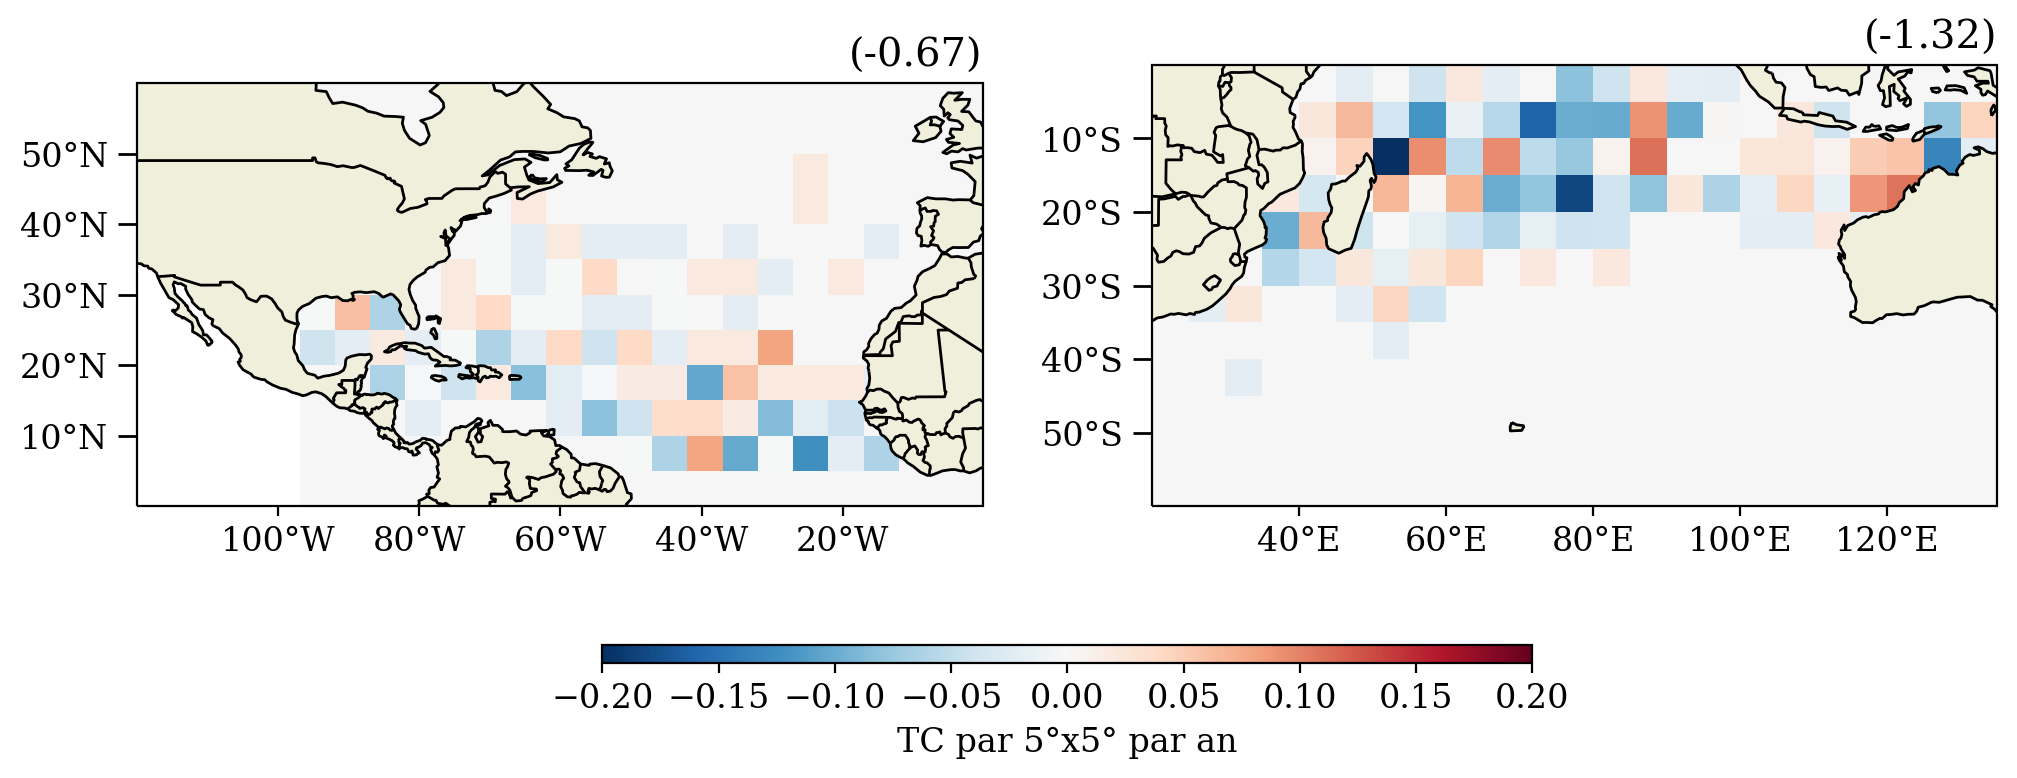
\includegraphics[width=\textwidth]{diff_density.png}
    \caption{Différences dans les densités de cyclogénèses détectées moyennes par \ang{5}$\times$\ang{5} et par an entre ATL-F et ATL-P (gauche) et SIO-F et
    SIO-P (droite). Les valeurs numériques entre parenthèses en haut à droite de chaque encadré présente la différence totale sur le bassin.}
    \label{fig:diff_track}
\end{figure}

Pour les deux expériences, la détection objective de TC dans les simulations indique une diminution de l'activité cyclonique, de \num{0.67} TC par an pour la
simulation faite sur le bassin NAtl, et de \num{1.32} TC par an pour celle faite sur le bassin SInd. Même sur une grille de \ang{5}$\times$\ang{5}, ces cartes
de différences demeurent bruitées, en raison de la fréquence d'occurrence relativement faible dans nos données. Dans le bassin SInd, une diminution forte est
notée entre \ang{70}E et \ang{80}E, tandis que l'activité semble augmenter au Nord-est de l'Australie. Dans le NAtl, la diminution semble plus marquée au sud du
bassin, notamment en dessous de \ang{15}N, du côté du continent Africain.

\subsection{Indices de cyclogénèse}

Nous calculons plusieurs indices de cyclogénèse pour analyser le changement annuel moyen entre les simulations du scénario RCP8.5 (ATL-F et SIO-F) et celles à
climat présent (ATL-P et SIO-P). En particulier, nous appliquons la régression de Poisson sur les champs ATL-P et SIO-P et ajustées sur les cyclogénèses
détectées dans ces simulations respectives. Les régressions sont faites avec l'humidité relative d'une part et le VPD d'autre part. Il s'agit donc du mode
opératoire de construction d'indices de cyclogénèse régionaux, si bien que ces derniers sont appelés LAM10 et LAVPD. Comme dans la \cref{sec:indice_ONI} et la
\cref{sec:indice_regional} avant cela, rappelons que ces deux indices sont caractérisés par des coefficients $b$ différents pour le bassin NAtl et SInd. Notons
d'ailleurs que nous ne faisons ici pas la distinction SIndW et SIndE, mais traitons le bassin SInd dans son ensemble.

Nous comparons également le changement future/présent par l'intermédiaire de l'indice LM10, dont les coefficients $b$ sont issus des champs ERA5 ajustés sur
IBTrACS. Notons que la régression LM10 est recalculée pour obtenir des coefficients à l'échelle du bassin SInd, plutôt que pour SIndW et SIndE séparément. Les
coefficients en résultant valent approximativement la moyenne des coefficients LM10 sur les deux sous-régions du bassin SInd (voir \cref{tab:coefs_fit_bassin}
du \cref{chap:chapitre_3}, \vpageref{tab:coefs_fit_bassin}). Enfin, le TCS est également utilisé à titre de référence. Le \cref{tab:coeffs_experiences} présente
(ou rappelle) les coefficients des indices sus-mentionnés.

\begin{table}[htpb]
    \centering
    \caption{Indices de cyclogénèse utilisés sur les expériences ATL et SIO}
    \label{tab:coeffs_experiences}
    \resizebox{\textwidth}{!}{
    \begin{tabular}{llrrrrrrr}
        \toprule\toprule
        \multicolumn{1}{l}{\textbf{Indice}} & \multicolumn{1}{l}{\textbf{Bassin}} & \multicolumn{6}{c}{\textbf{Coefficients}} & \multicolumn{1}{c}{\textbf{Calibration}} \\
        \midrule
                                            & & $b_0$ & $b_{\eta}$ & $b_{V_{\mathrm{shear}}}$ & $b_H$ & $b_s$ & $b_T$ & \\
        \midrule
        \multirow{2}{*}{LAVPD} & NAtl & \num{-216.0074} & \num{56.4265} & \num{-0.0511} & --- & \num{-0.0369} & \num{0.3901} & \num{1.048} \\
                               & SInd & \num{-256.6651} & \num{67.4970} & \num{-0.0384} & --- & \num{-0.0420} & \num{0.3506} & \num{1.021} \\ 
        \midrule
        \multirow{2}{*}{LAM10} & NAtl & \num{-254.8083} & \num{66.6267} & \num{-0.0551} & \num{0.0065} & --- & \num{0.3719} & \num{1.050}\\
                               & SInd & \num{-233.9484} & \num{60.8866} & \num{-0.0375} & \num{0.0155} & --- & \num{0.2876} & \num{1.022} \\
        \midrule
        \multirow{2}{*}{LM10}  & NAtl & \num{-17.3713} & \num{2.1677} & \num{-0.0594} & \num{0.0651} & --- & \num{0.3313}  & \num{0.055}\\
                               & SInd & \num{-15.9070} & \num{1.7221} & \num{-0.0691} & \num{0.0672} & --- & \num{0.4758} & \num{0.050}\\
        \midrule
        \multirow{2}{*}{TCS}   & NAtl    & \num{-5.8} & \num{1.03} & \num{-0.15} & \num{0.05} & --- & \num{0.56} & \num{1.389e-4}\\
                               & SInd    & \num{-5.8} & \num{1.03} & \num{-0.15} & \num{0.05} & --- & \num{0.56} & \num{1.335e-4}\\
        \bottomrule
    \end{tabular}
}
\end{table}

Pour le calcul des indices sur les simulations en climat présent, un coefficient de calibration est appliqué pour ramener les indices vers la moyenne annuelle
(entre juillet et juin pour le bassin SInd) du nombre de TC déterminé par le schéma de détection, après application du filtre du STJ. Pour l'application des
indices aux simulations RCP8.5, les coefficients de calibration utilisés pour le climat présent sont ré-employés tels quels. Ces coefficients sont précisés dans
le \cref{tab:coeffs_experiences}.

Remarquons que les indices LAVPD et LAM10 présentent des valeurs $b_0$ et $b_\eta$ inhabituelles par rapport à celles rencontrées jusqu'à maintenant. Ces
valeurs sont propres aux simulations et cyclogénèses de référence sur lesquelles sont faites les régressions et ne sauraient s'interpréter ---~dans le cas de
$b_\eta$~--- comme un biais septentrional extrême par rapport à LM10. Il semble en outre crédible que les fortes valeurs de $b_\eta$ permettent de compenser les
valeurs $b_0$ remarquablement basses, de façon à ce que la fréquence annuelle moyenne de ces indices soient proches de celle détectée par le schéma de
détection. Il n'est en effet quasiment pas nécessaire de recalibrer un indice pour l'appliquer aux mêmes données dont sont issues ses coefficients $b$, comme en
attestent les coefficients de calibration proches de l'unité pour LAM10 et LAVPD. En revanche, la valeur $b_\eta^{\mathrm{LAM10}} > b_\eta^{\mathrm{LAVPD}}$
pour le bassin NAtl indique bel et bien un décalage de l'activité simulée vers des latitudes légèrement supérieures pour LAM10 par rapport à LAVPD. Dit
autrement, ces coefficients ne peuvent être comparés que lorsqu'ils sont été obtenus dans des conditions comparables.

\subsection{Changements futurs}

La \cref{fig:delta_F_P} présente les changements moyens, exprimés en TC par \ang{1}$\times$\ang{1} par an. Tous les indices, y compris le TCS, indiquent un une
diminution de l'activité cyclonique annuelle moyenne dans les simulations RCP8.5 par rapport aux simulations en climat présent. Ici, tous les indices utilisés
projettent une diminution de l'activité cyclonique, dont l'ampleur varie entre \num{-0.22} TC par an et \num{-0.68} TC par an dans l'expérience ATL, et entre
\num{-0.58} TC par an et \num{-1.68} TC par an dans l'expérience SIO.

\begin{figure}[htbp]
    \centering
    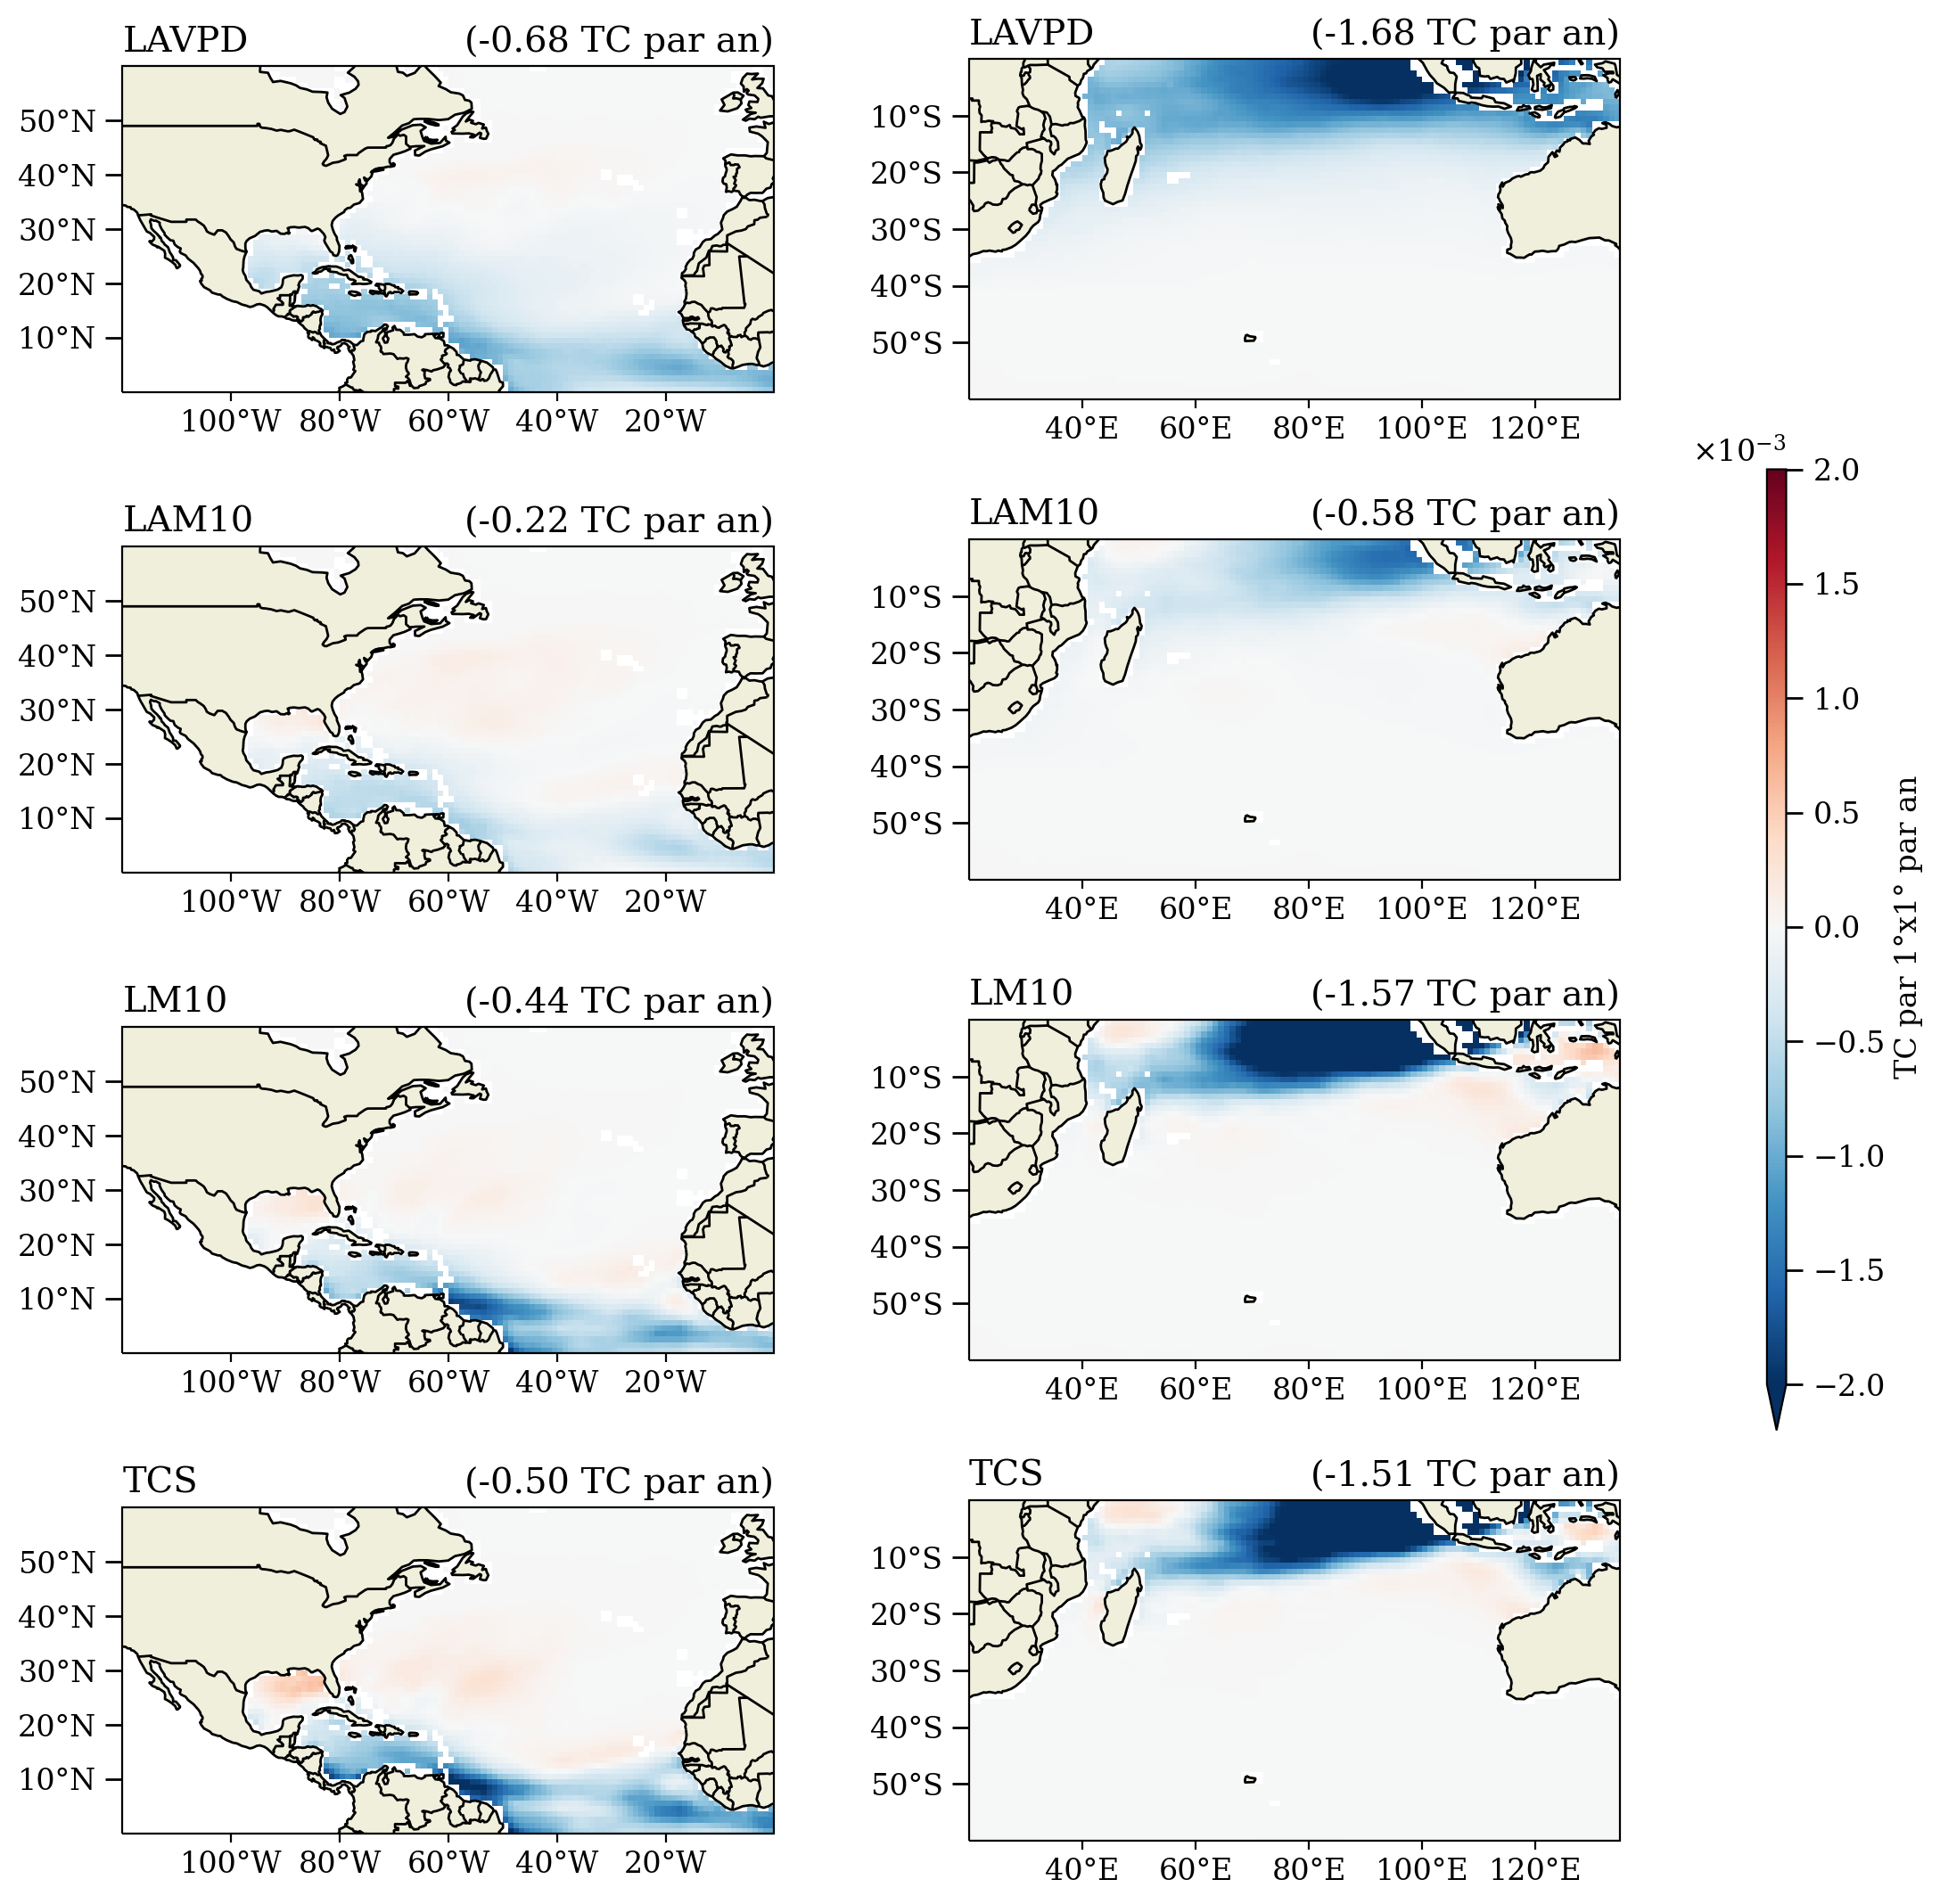
\includegraphics[width=\textwidth]{delta_F_P.png}
    \caption{Cartes des différences annuelles moyennes entre ATL-F et ATL-P (colonne de gauche) et entre SIO-F et SIO-P (colonne de droite), pour les indices
    décrits dans le \cref{tab:coeffs_experiences}. L'intégrale sur le domaine est renseignée en haut à droite de chaque encadré, entre parenthèses.}
    \label{fig:delta_F_P}
\end{figure}

La diminution de l'activité constatée pour tous les indices construits par régression de Poisson, notamment ceux basés sur l'humidité relative à \hPa{600}, y
compris le TCS est ici d'ordre circonstanciel. Si il est en effet avéré que les indices de cyclogénèse classiquement utilisés dans la littérature projettent
généralement une augmentation de l'effet cyclonique, ce qui inclue notamment le TCS, ces projections sont susceptibles de varier pour différents modèles de
climat, différentes expériences, et pour différents bassins d'activité. \textcite{camargo_testing_2014} montrent par exemple à travers des simulations réalisées
avec le modèle HiRAM du GFDL \parencite{zhao_simulations_2009} et forcés par des SST issues d'autres modèles couplés, que certaines simulations indiquent une
diminution de l'activité dans ces régions, pour des indices dérivés du TCS à l'échelle globale. Par ailleurs, dans \textcite{cattiaux_projected_2020} ---~étude
dont les simulations SIO-P et SIO-F utilisées ici sont tirées~--- si la moyenne des trois indices que sont le TCS, le GPI et le CYGP indique une augmentation à
l'échelle du bassin SInd, le TCS pris individuellement indique une légère diminution. On s'intéresse alors ici plus spécifiquement aux différences dans les
projections entre les divers indices.

Les deux indices basés sur des réanalyses, à savoir le TCS et LM10, présentent tous deux des réponses très similaires dans les scénarios futurs, aussi bien
spatialement que dans leur amplitude. Ces deux indices présentent notamment, dans les deux expériences, une diminution plus importante que LAM10, lequel est
basé sur la même combinaison de prédicteurs. Dans le bassin SInd, la réponse est caractérisée par une forte diminution dans toute la partie centrale, entre
\ang{60}E et \ang{100}E, entre l'équateur et \ang{20}S. Une légère augmentation est constatée à l'extrémité Nord-ouest du bassin. Une très légère mais possible
augmentation est notée dans le canal du Mozambique, à \ang{20}S. Les indices LM10 et TCS se distinguent quelque peu par la réponse indiquée le long des côtes
Australiennes. En effet, si une réduction de l'activité semble dominer dans le TCS, notamment en Mer de Timor, celle-ci semble moins prononcée dans LM10.

Dans le bassin NAtl, les deux indices concentrent l'ensemble de la diminution de l'activité dans la Mer des Caraïbes et entre l'Amérique centrale et le
continent Africain, en dessous de \ang{15}N. Tous deux indiquent toutefois une augmentation dans le Golfe du Mexique. Qu'il s'agisse du TCS ou de LM10, la
réponse spatiale dans les deux indices semble partager certaines caractéristiques avec le changement dans les densités de cyclogénèses détectées dans ces
simulations (voir \cref{fig:diff_track}), plus particulièrement pour le bassin SInd. L'indice LAM10 présente quant à lui pour les deux bassins la même
répartition spatiale que LM10 et TCS, mais d'une ampleur réduite. Bien que ressemblantes, LAM10 semble être légèrement plus proche du TCS que de LM10, notamment
pour ce qui est de la diminution côté Australien dans le SInd, ainsi que dans le signal noté le long du continent Africain, au sud de la Mauritanie.

L'introduction du VPD dans la régression, via l'indice LAVPD présente deux effets notables. Le premier d'entre eux concerne l'amplitude de la réponse suggérée
par l'indice dans le scénario RCP8.5. LAVPD présente en effet dans les deux bassins la réduction la plus forte, avec \num{-0.68} TC par an dans le bassin NAtl,
et \num{-1.68} TC par an dans le SInd. Le deuxième élément concerne la signature spatiale de la réponse. Le remplacement de l'humidité relative par le VPD se
traduit en effet par une diminution très nettement plus homogène sur les deux bassins. En particulier, le SInd ne présente plus de signe d'augmentation autour
de l'Australie de part et d'autre de la Mer de Timor, ni d'augmentation au dessus de l'île de Madagascar. Dans le NAtl, la diminution est lisse dans l'ensemble
de la MDR, et le Golfe du Mexique ne présente plus non plus de signe d'augmentation.

\subsection{Conclusion}

Dans cette section, nous avons appliqué plusieurs indices de cyclogénèse à deux expériences réalisées avec le modèle ARPEGE-Climat dans sa configuration
basculée-étirée, chacune avec une simulation en climat présent et une autre sous le scénario RCP8.5. Une des expériences porte sur le bassin Nord-Atlantique
\parencite{chauvin_future_2020}, tandis que l'autre est centrée sur la région SInd \parencite{cattiaux_projected_2020}. L'objectif de l'analyse consistait à
étudier l'effet de l'introduction du VPD dans la réponse au réchauffement climatique projetée par un indice de cyclogénèse. En particulier, l'indice contenant
le VPD fut construit manière régionale à partir des deux simulations à climat présent (LAVPD), de façon à bénéficier d'un indice mieux adapté à notre jeu de données,
comme le montre la \cref{sec:indice_regional} du \cref{chap:chapitre_3}.

Comme pour les \cref{sec:indice_ONI,sec:tendances_VPD}, le filtre du STJ est appliqué aux trajectoires détectées dans les quatre simulations, dont les premières
échéances sont conservées et assimilées aux cyclogénèses. Les densités de cyclogénèses détectées indiquent une diminution de l'activité cyclonique pour les deux
bassins, environ deux fois plus forte pour le bassin SInd que pour le bassin NAtl. De manière similaire, tous les indices utilisés ici, à savoir LAVPD, LAM10
---~une version locale de l'indice AM10 et construit sur les simulations climat présent des expériences en configuration basculée-etirée~--- LM10 et TCS
indiquent également une diminution de l'activité dans la simulation faite sous le scénario RCP8.5. La diminution constatée pour les indices dérivés du TCS, et
plus particulièrement ceux étant fonction de l'humidité relative à \hPa{600}, apparaît ici comme une caractéristique propre à notre modèle et à ces expériences
spécifiques. Une analyse multimodèles et globale serait en effet nécessaire pour évaluer de manière plus fiable le signe de la réponse des différents indices.

Il est possible de tirer deux constats principaux de cette étude. Le premier est d'une part que, dans nos expériences, l'introduction du VPD amplifie la
diminution de l'activité cyclonique dans la simulation à climat plus chaud, tandis que d'autre part, le VPD produit un signal beaucoup plus homogène que les
indices utilisant l'humidité relative à \hPa{600}. Le second constat est que, dans ces expériences, le TCS et son dérivé LM10 semblent présenter une réponse
plus proche de celle mesurée par le schéma de détection. L'amplitude de la diminution est en effet proche de celle mesurée par le traqueur dans les deux
bassins. Les réponses spatiales du TCS, LM10 et LAM10 présentent en outre plus de similarités avec le changement dans la densité de cyclogénèses mesurées par le
traqueur que l'indice LAVPD. Ces résultats, combinés à ceux de \textcite{cattiaux_projected_2020,chauvin_future_2020} montrant notamment que le GPI et le CYGP
indiquent une réponse opposée dans ces mêmes simulations, justifient alors d'autant plus l'utilisation du TCS et de ses dérivés (c'est à dire la re-détermination
des coefficients associés à ses prédicteurs) pour les applications en climat futur, en plus des avantages que ce dernier présente, à savoir sa reproductibilité
et son interprétabilité.

%--------------------------------------
\section{Synthèse}

Dans ce chapitre, l'effet de l'introduction de nouveaux prédicteurs dans des indices de cyclogénèse construits par régression de Poisson est évalué. Faisant
suite aux résultats du \cref{chap:chapitre_3}, dans lequel il est montré que la variabilité interannuelle des indices construits selon ce modèle statistique est
extrêmement robuste aux perturbations de leurs coefficients, une première partie s'est consacrée à la construction d'un indice dans lequel un indice ENSO (ONI)
est introduit et ajouté aux prédicteurs déjà présents, avec l'objectif de parvenir à améliorer la représentation de la variabilité interannuelle inférée par
l'indice. Spécifiquement, le prédicteur est construit en répliquant en tout point de l'espace l'anomalie de SST pour un pas de temps de donné, de façon à
contraindre le modèle statistique à simuler l'effet de l'ENSO sur la variabilité temporelle de la fréquence modélisée. En effet, si le TCS et ses dérivés
semblent déjà reproduire quelques pics d'activité historique liés à ce mode de variabilité, seuls les évènements les plus importants semblent laisser une
empreinte dans la variabilité inférée par ceux-ci. L'introduction explicite d'un indice ENSO dans la régression laisse alors espérer une réponse plus
consistante aux phases de l'ENSO, notamment pour des évènements d'ampleur moindres.

Étant donnée la nature de l'impact de l'ENSO sur l'activité cyclonique tropicale, à savoir présentant un effet positif dans les bassins de l'océan Pacifique, et
négatif dans l'océan Indien sud ainsi que dans l'Atlantique nord, un tel indice ne peut être défini à l'échelle globale et n'a donc de sens que dans une
démarche de régionalisation de l'indice, selon le mode opératoire de construction d'un indice régional décrit dans la \cref{sec:indice_regional} du
\cref{chap:chapitre_3}, nommé LOA. Les régressions statistiques locales rejettent le nouveau prédicteur dans la plupart des bassins océaniques, à l'exception
des bassins WPac et SPac. Cela se traduit par un intervalle de confiance à \prct{95} pour les coefficients $b$ associés à l'ONI à cheval autour de \num{0}, ou
autrement dit que le signe du coefficient, et donc de la sensibilité de la fréquence modélisée à l'ONI, n'est pas significativement déterminé.

Toutefois, dans la plupart des régions où le coefficient n'est pas significatif, la valeur suggérée apparaît en accord avec le lien constaté dans le modèle
entre l'activité cyclonique détectée et l'indice ONI. Il apparaît par ailleurs qu'en dépit de la non-significativité des coefficients, la variabilité
interannuelle inférée par le nouvel indice régional s'en trouve néanmoins sensiblement améliorée. En particulier, la corrélation entre la variabilité
interannuelle simulée et celle détectée par le schéma de détection est rendue statistiquement significative dans tous les bassins océaniques au seuil de
\prct{95} lorsque l'indice ONI est introduit, à l'exception du bassin NAtl, qui est néanmoins nettement plus proche du seuil que les indices n'incluant pas ce
prédicteur.

Le paradoxe apparent entre le rejet du prédicteur d'une part et l'amélioration sensible de la variabilité interannuelle d'autre part peut s'expliquer par le
fait que la régression de Poisson vise avant toute chose à identifier la combinaison log-linéaire de prédicteurs permettant d'expliquer la meilleure répartition
de l'activité cyclonique. Les prédicteurs usuels de grande échelle tendent à présenter une variabilité spatiale plus importante que leur variabilité temporelle,
ce qui contribue probablement à ce que ces indices excellent dans la répartition géographique de l'activité simulée au détriment de la variabilité temporelle.
Le prédicteur ONI, au contraire, n'est que pure variabilité temporelle, puisque constant dans l'espace par construction. Ainsi le rejet de l'ONI dans la
régression exprime vraisemblablement l'impossibilité de mettre en relation la variabilité spatiale de l'activité détectée dans le modèle avec le prédicteur ONI.
Cela laisse entendre que la méthodologie de la régression de Poisson n'est pas la plus adaptée pour espérer améliore d'avantage la variabilité interannuelle
inférée par les indices. L'utilisation de modèles statistiques plus sophistiqués pourrait peut-être apporter une solution à ce problème, tels que les modèles
dits \textquote{hurdle}. Les modèles de cette famille consistent en fait en la combinaison de deux processus, l'un visant à évaluer la probabilité d'avoir une
occurrence de TC de façon binaire, et l'autre visant à déterminer l'amplitude de l'évènement, c'est à dire le nombre de TC, sachant qu'il y a occurrence.

L'utilisation de l'ONI dans un indice de cyclogénèse dégrade quelque peu l'interprétabilité physique de l'indice, puisque l'indice ENSO ne fait pas directement
partie des ingrédients à priori importants pour que le processus de cyclogénèse ait lieu. Toutefois, ce genre de produit hybride pourrait potentiellement avoir
de l'intérêt pour la prévision opérationnelle de l'activité cyclonique.

Une seconde partie du chapitre s'est consacrée au remplacement de l'humidité relative à \hPa{600} dans la régression par le déficit de saturation d'humidité
intégré sur la colonne atmosphérique, ou VPD. Cette variable présente en effet l'avantage, par rapport à l'humidité relative, de changer d'amplitude avec le
réchauffement climatique, alors que l'humidité relative est projetée approximativement constante. Par ailleurs, la littérature suggère que le VPD serait une
variable plus pertinente que l'humidité relative dans le processus de cyclogénèse. L'introduction du VPD accorde dans la régression plus de poids à la SST
relative, lequel voit son coefficient augmenter. Cet effet est robuste entre la simulation ARPEGE forcée par HadISST1, ERA5 et ainsi que dans la littérature.
Comme pour on pouvait s'y attendre, l'utilisation du VPD en lieu et place de l'humidité relative ne présente aucun impact clair sur la variabilité interannuelle,
dans un sens ou dans l'autre.

Néanmoins, l'indice construit avec le VPD (AVPD) réduit des biais positifs présents sinon dans tous les indices qui sont définis comme fonction de l'humidité
relative. L'effet est le plus notable dans la Mer Rouge et dans le Golfe Persique, si bien qu'un indice dans la Mer Rouge, le Golfe Persique, ainsi que dans
dans l'océan Atlantique Sud au large de l'Angola. L'utilisation du VPD en remplacement de l'humidité relative est donc à minima particulièrement recommandée
pour l'application d'indices de cyclogénèse dans le bassin NInd.

À défaut de se démarquer par leur représentation de la variabilité interannuelle, les indices basés sur le VPD, qu'ils soient établis sur les champs modèle ou
bien de la réanalyse ERA5, se distinguent également de ceux basés sur l'humidité relative à travers les différences notées dans l'analyse des tendances dans le
décompte du nombre de TC sur la période historique. De manière la plus notable, tous les indices basés sur l'humidité relative indiquent une tendance à la
hausse statistiquement significative de l'ordre de quelques TC par décennie, dans le modèle comme dans la réanalyse. Une telle tendance n'est pas constatée par
le schéma de détection ou dans les observations historiques. L'introduction du VPD permet alors d'annuler cette tendance, et offre par cette occasion une
meilleure cohérence avec la mesure directe par détection objective ainsi qu'avec IBTrACS. Ainsi, la convergence entre l'approche directe par détection objective
et l'approche indirecte des indices de cyclogénèse notée par \textcite{camargo_testing_2014} dans des scénarios climatiques futurs lorsque le VPD est introduit
semble également avoir ici une empreinte sur la période historique.

Par ailleurs, l'application d'un indice de cyclogénèse basé sur le VPD à des simulations climatiques sous le scénario RCP8.5 montre que l'utilisation du VPD
amplifie la réduction de l'activité cyclonique constatée par les indices basés sur l'humidité relative. Dans ces simulations, le VPD tend également à lisser la
réponse spatiale en produisant une réduction homogène à l'échelle des deux bassins océaniques considérés. Dans ces simulations, le TCS et son dérivé régional
défini sur la simulation à climat présent présentent toutefois une réponse qui semble en meilleur accord avec le signal indiqué par le schéma de détection, par
rapport à l'indice utilisant le VPD. Si la diminution constatée de l'activité cyclonique dans ces simulations avec le TCS est probablement le résultat d'un
concours de circonstances propre à ces régions et à ces simulations, ce résultat fournit néanmoins une raison supplémentaire ---~en plus de ses qualités déjà
mentionnées dans le \cref{chap:chapitre_3}, notamment dans la \cref{sec:proprietes_indices}~--- de porter une attention plus particulière à cet indice par
rapport notamment au GPI, dont l'usage est très largement répandu.

\end{document}
